\documentclass[11pt,a4paper]{article}

% ---------------------------------------------------------------- packages
\usepackage[T1]{fontenc}
\usepackage[utf8]{inputenc}
\usepackage{lmodern}
\usepackage[margin=2.4cm]{geometry}
\usepackage{microtype}
\usepackage{amsmath,amssymb}
\usepackage{graphicx}
\usepackage{booktabs}
\usepackage{multirow}
\usepackage{tabularx}
\usepackage{array}
\usepackage{xcolor}
\usepackage{enumitem}
\usepackage{float}
\usepackage[font=small,labelfont=bf]{caption}
\usepackage{listings}
\usepackage{tikz}
\usetikzlibrary{arrows.meta,positioning,fit,calc,backgrounds}
\usepackage{fancyhdr}
\usepackage[hidelinks]{hyperref}

\graphicspath{{../results/figures/}{figures/}}

\definecolor{accent}{HTML}{2A78D6}
\definecolor{ink2}{HTML}{52514E}
\definecolor{codebg}{HTML}{F4F5F8}
\definecolor{kw}{HTML}{1F4E9C}
\definecolor{str}{HTML}{B4461D}
\definecolor{cmt}{HTML}{6B7280}

\lstdefinelanguage{OmniQL}{
  morekeywords={SEARCH,WHERE,AND,OR,NOT,IN,BETWEEN,IS,NULL,FUSE,RRF,WEIGHTED,AUTO,LIMIT,WITH,EXPLAIN,ANALYZE,
                MATCH,SIMILAR,CONTAINS,IMAGE,AUDIO,DOC,VECTOR},
  sensitive=true, morecomment=[l]{--}, morestring=[b]'
}
\lstset{
  basicstyle=\ttfamily\small, columns=fullflexible, keepspaces=true, backgroundcolor=\color{codebg},
  frame=single, framerule=0pt, framesep=6pt, xleftmargin=6pt, xrightmargin=6pt, aboveskip=8pt, belowskip=8pt,
  keywordstyle=\color{kw}\bfseries, stringstyle=\color{str}, commentstyle=\color{cmt}\itshape,
  breaklines=true, showstringspaces=false
}

\setlist{itemsep=2pt,topsep=4pt}
\setlength{\parskip}{3pt}
\renewcommand{\arraystretch}{1.12}
\newcolumntype{L}{>{\raggedright\arraybackslash}X}

\pagestyle{fancy}
\fancyhf{}
\fancyhead[L]{\small\color{ink2}OmniSearch: a cost-based multimodal hybrid search engine}
\fancyhead[R]{\small\color{ink2}\thepage}
\renewcommand{\headrulewidth}{0.3pt}

\newcommand{\code}[1]{\texttt{\small #1}}
\newcommand{\fig}[1]{Figure~\ref{#1}}
\newcommand{\tab}[1]{Table~\ref{#1}}
\newcommand{\sect}[1]{Section~\ref{#1}}

% ---------------------------------------------------------------- title
\title{\vspace{-1.2cm}\textbf{OmniSearch}\\[4pt]
  \large A Cost-Based Multimodal Hybrid Search Engine\\[2pt]
  \normalsize Keyword + vector retrieval over text, images, audio and video, with structured filters,\\
  a query language, a cost-based optimizer and instance-optimal top-$k$ fusion}
\author{Srinjoy Das\\[1pt] \small Roll No.\ 22CS30054\\[4pt] \small Advanced Database Systems --- Course Project Report}
\date{\small October 2026}

\begin{document}
\maketitle
\thispagestyle{empty}

\begin{abstract}
\noindent
Keyword search misses meaning, vector search misses exact terms, and real collections mix text, images,
audio and video with structured attributes. OmniSearch is a hybrid retrieval engine that treats this as a
\emph{database} problem. Every modality is turned into searchable text (OCR, captions, transcripts) and
into vectors, stored in purpose-built indexes, and queried through OmniQL, a small declarative language.
A cost-based optimizer chooses the access path for each clause, and an instance-optimal top-$k$
algorithm fuses the ranked lists. All of it is implemented from scratch in Python and numpy (about
5{,}700 lines, 100 tests): a compressed inverted index with BM25 and WAND; HNSW and IVF vector indexes
with SQ8 and product quantization; bitmap and B$^+$-tree attribute indexes with equi-depth histograms;
and Fagin's Threshold Algorithm and NRA. Experiments against FAISS and SQLite FTS5 show three things.
First, the calibrated optimizer tracks the best filtered-vector access path across a $1000\times$ range
of filter selectivity, avoiding plans that are up to $540\times$ slower, with recall 1.00 at every
point. Second, the Threshold Algorithm returns the \emph{exact} weighted top-$k$ while fixed-depth fusion
loses up to 31\% of it. Third, equi-depth histograms with most-common values keep selectivity estimates
within a median q-error of 1.00, against a maximum of 802 for equi-width histograms. A retrieval-quality
study on a 268-item multimodal collection shows that no single retrieval path wins. Keyword search falls
to nDCG@10 0.12 on typos and 0.50 on noisy OCR text, where character-$n$-gram vectors reach 0.87 and 1.00.
Fusion recovers most of that gap, and score-aware fusion is more robust than rank-only RRF.
\end{abstract}

\tableofcontents
\newpage

% =====================================================================
\section{Introduction}
\label{sec:intro}

Search over a modern collection, such as a product catalogue, a lecture archive or a photo library, asks
for three kinds of matching at once. A user typing \emph{``zenith sneaker''} wants the exact brand
token matched (\emph{lexical} matching). A user typing \emph{``sneakr''} or \emph{``shoe for running''}
wants the meaning matched (\emph{semantic} matching). Both usually come with predicates such as
\emph{price $<$ 100} or \emph{category = sneakers} (\emph{structured} filtering). The content is often
not text at all: a brand name printed on a product photo, a phrase on a lecture slide or words spoken
in a clip.

Production systems answer this with two separate engines, a full-text engine and a vector database, glued
together in application code. The interesting questions are then exactly the ones a database course is
about, and the glue hides them:
\begin{itemize}
  \item \textbf{Access-path selection.} With a selective filter, should a vector query scan the few
        qualifying rows exactly, search an ANN graph while skipping disallowed nodes, or search
        unfiltered and post-filter? The answer flips with selectivity and with the
        \emph{correlation} between the filter and the query.
  \item \textbf{Selectivity estimation.} The choice above needs an estimate of the filter's
        selectivity, which needs statistics.
  \item \textbf{Top-$k$ aggregation.} Combining several ranked lists into one top-$k$ is the classic
        middleware problem studied by Fagin et al.~\cite{fagin2001}. Fixed-depth fusion is fast but
        not exact.
\end{itemize}

\paragraph{Contributions.} OmniSearch implements the full stack, so each of these questions can be
answered by experiment:
\begin{enumerate}
  \item A \textbf{data model and query language} (OmniQL) that mixes scoring clauses (\code{MATCH},
        \code{SIMILAR}) with SQL-style filters under three-valued logic (\sect{sec:model}).
  \item \textbf{Index structures built from scratch}: a gap + variable-byte compressed inverted index
        with BM25 and WAND; HNSW and IVF vector indexes with SQ8 and PQ compression and multi-vector
        MaxSim for video; and bitmap, B$^+$-tree and histogram attribute indexes (\sect{sec:storage}).
  \item A \textbf{cost-based optimizer} whose unit costs are calibrated on the host machine. It
        chooses filtered-vector plans, B$^+$-tree vs.\ column scan, BM25 vs.\ WAND, and the top-$k$
        algorithm, and explains its choices with \code{EXPLAIN ANALYZE} (\sect{sec:optimizer}).
  \item \textbf{Exact top-$k$ fusion} with the Threshold Algorithm and NRA, alongside reciprocal-rank
        fusion (\sect{sec:fusion}).
  \item An \textbf{experimental evaluation} against FAISS and SQLite FTS5, plus a retrieval-quality
        study that separates the lexical, semantic and OCR paths (\sect{sec:eval}).
\end{enumerate}

% =====================================================================
\section{Background and related work}
\label{sec:related}

\paragraph{Lexical retrieval.} BM25~\cite{bm25} scores a document $d$ for query terms $q_i$ as
\begin{equation}
  \mathrm{BM25}(d,q) = \sum_{i} \mathrm{IDF}(q_i)\,
  \frac{f(q_i,d)\,(k_1+1)}{f(q_i,d) + k_1\left(1-b+b\,\frac{|d|}{\mathrm{avgdl}}\right)},
  \qquad \mathrm{IDF}(q_i) = \ln\!\left(1 + \frac{N - n_i + 0.5}{n_i + 0.5}\right),
\end{equation}
with $k_1 = 1.2$ and $b = 0.75$ in OmniSearch. WAND~\cite{wand} skips documents whose score upper bound
cannot reach the current top-$k$ threshold.

\paragraph{Approximate nearest neighbours.} HNSW~\cite{hnsw} builds a multi-layer proximity graph and
answers queries with a greedy beam search of width $ef$. IVF partitions vectors with $k$-means and
scans the $nprobe$ closest partitions. Product quantization~\cite{pq} compresses vectors into
sub-space codebook indices and computes distances from lookup tables.

\paragraph{Filtered vector search.} Milvus~\cite{milvus} and AnalyticDB-V~\cite{adbv} combine
attribute filtering with ANN search and pick between pre- and post-filtering by cost. ACORN~\cite{acorn}
changes the HNSW construction itself so in-graph filtering stays efficient for arbitrary predicates.
OmniSearch takes the optimizer route and measures where each plan breaks.

\paragraph{Rank aggregation.} Reciprocal Rank Fusion (RRF)~\cite{rrf} merges lists by rank only:
$\mathrm{RRF}(d) = \sum_i w_i/(k + r_i(d))$ with $k=60$. For score-based (weighted) fusion, Fagin's
Threshold Algorithm (TA) and No-Random-Access algorithm (NRA)~\cite{fagin2001} are instance-optimal for
monotone aggregation functions.

\paragraph{Access-path selection.} The optimizer follows the System R tradition~\cite{selinger}: an
explicit cost model with unit costs (cf.\ PostgreSQL's \code{seq\_page\_cost} and
\code{cpu\_tuple\_cost}), statistics-driven selectivity estimates, and a choice of the cheapest
alternative per operator.

\paragraph{Multimodal encoders.} With the optional neural profile, CLIP~\cite{clip} maps images, video
keyframes and text into one embedding space, BLIP produces captions, Whisper transcribes speech and
RapidOCR (PP-OCR) reads text in images and video frames.

% =====================================================================
\section{System overview}
\label{sec:overview}

\begin{figure}[t]
\centering
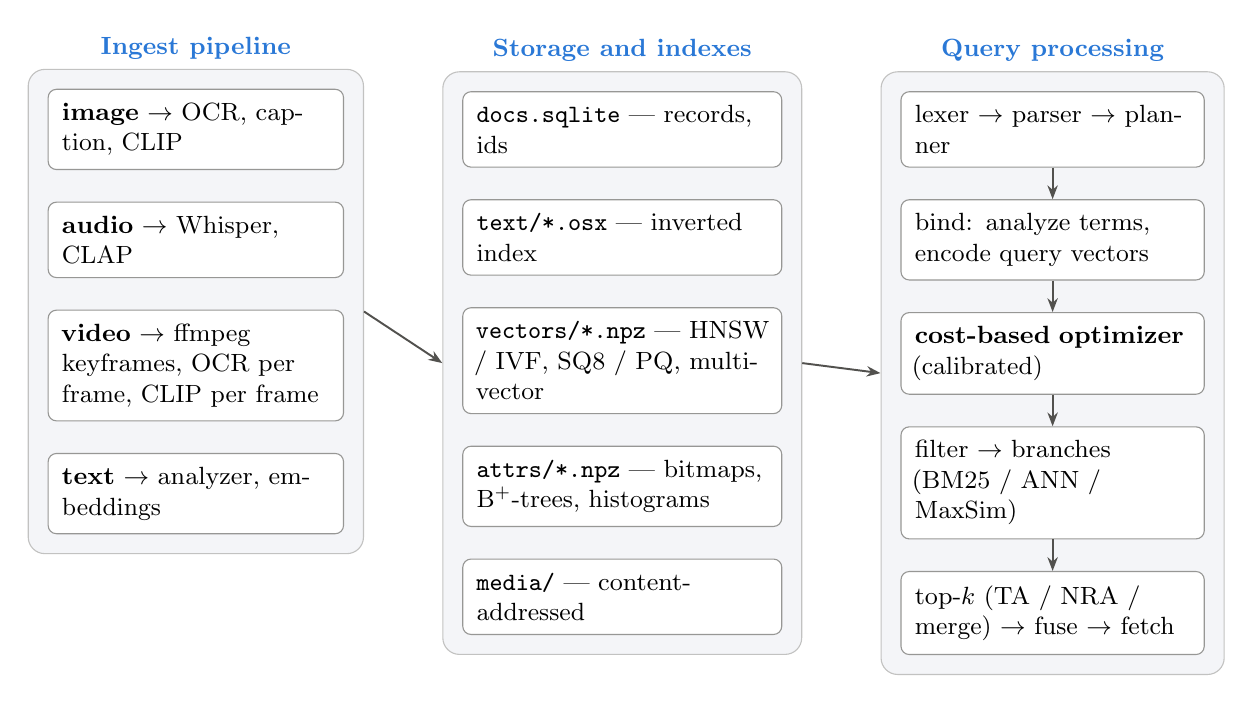
\begin{tikzpicture}[
  font=\small, node distance=4mm and 6mm,
  box/.style={draw=ink2!60, rounded corners=3pt, fill=white, align=left, inner sep=5pt, text width=#1},
  box/.default=3.4cm,
  group/.style={draw=ink2!35, rounded corners=6pt, fill=codebg, inner sep=7pt},
  title/.style={font=\small\bfseries, text=accent},
  arr/.style={-{Stealth[length=5pt]}, draw=ink2, line width=0.7pt}
]
% ingest
\node[box] (img) {\textbf{image} $\rightarrow$ OCR, caption, CLIP};
\node[box, below=of img] (aud) {\textbf{audio} $\rightarrow$ Whisper, CLAP};
\node[box, below=of aud] (vid) {\textbf{video} $\rightarrow$ ffmpeg keyframes, OCR per frame, CLIP per frame};
\node[box, below=of vid] (txt) {\textbf{text} $\rightarrow$ analyzer, embeddings};
% storage
\node[box=3.7cm, right=15mm of img] (docs) {\code{docs.sqlite} --- records, ids};
\node[box=3.7cm, below=of docs] (inv) {\code{text/*.osx} --- inverted index};
\node[box=3.7cm, below=of inv] (vec) {\code{vectors/*.npz} --- HNSW / IVF, SQ8 / PQ, multi-vector};
\node[box=3.7cm, below=of vec] (att) {\code{attrs/*.npz} --- bitmaps, B$^+$-trees, histograms};
\node[box=3.7cm, below=of att] (med) {\code{media/} --- content-addressed};
% query
\node[box=3.5cm, right=15mm of docs] (parse) {lexer $\rightarrow$ parser $\rightarrow$ planner};
\node[box=3.5cm, below=of parse] (bind) {bind: analyze terms, encode query vectors};
\node[box=3.5cm, below=of bind] (opt) {\textbf{cost-based optimizer} (calibrated)};
\node[box=3.5cm, below=of opt] (exec) {filter $\rightarrow$ branches (BM25 / ANN / MaxSim)};
\node[box=3.5cm, below=of exec] (fuse) {top-$k$ (TA / NRA / merge) $\rightarrow$ fuse $\rightarrow$ fetch};
\begin{scope}[on background layer]
\node[group, fit=(img)(aud)(vid)(txt), label={[title]above:Ingest pipeline}] (G1) {};
\node[group, fit=(docs)(inv)(vec)(att)(med), label={[title]above:Storage and indexes}] (G2) {};
\node[group, fit=(parse)(bind)(opt)(exec)(fuse), label={[title]above:Query processing}] (G3) {};
\end{scope}
\draw[arr] (G1.east) -- (G2.west);
\draw[arr] (G2.east) -- (G3.west);
\draw[arr] (parse) -- (bind); \draw[arr] (bind) -- (opt); \draw[arr] (opt) -- (exec); \draw[arr] (exec) -- (fuse);
\end{tikzpicture}
\caption{Architecture. Every modality is reduced to text (searched with BM25) and to vectors (searched
with ANN indexes); attributes go to bitmap / B$^+$-tree indexes with statistics. A query is parsed,
bound, optimized with calibrated costs, and executed as filter $\rightarrow$ scoring branches
$\rightarrow$ top-$k$ fusion.}
\label{fig:arch}
\end{figure}

\fig{fig:arch} shows the three layers. The \textbf{ingest pipeline} routes each media field to
extractors and encoders, batching model calls. Precomputed values (for example captions and vectors
computed separately on a GPU) are reused, so expensive models never have to run on the indexing
machine. The \textbf{storage layer} keeps records in SQLite, which maps dense internal document ids
to external ids, and keeps every index in its own file format. The \textbf{query layer} turns OmniQL
into a physical plan, executes it and can report estimated versus actual cost for every operator.

Two encoder profiles are provided. The \emph{classic} profile is fully offline: hashed character
$n$-gram text vectors, colour-layout image vectors and OCR. It needs no model downloads and is used
for every experiment in this report. The \emph{CLIP} profile adds CLIP image and keyframe embeddings,
BLIP captions and Whisper transcripts, so a text query can match pixels directly.

% =====================================================================
\section{Data model and query language}
\label{sec:model}

\paragraph{Schema.} A collection's schema declares typed fields:
\begin{itemize}
  \item \textbf{media} fields (image, audio, video) with a list of extractors (\code{ocr},
        \code{caption}, \code{transcript});
  \item \textbf{text} fields, the concatenation of source fields such as
        \code{title}, \code{description} and \code{image.ocr};
  \item \textbf{vector} fields with an encoder, a source and an index type (\code{hnsw}, \code{ivf},
        \code{flat});
  \item \textbf{multi-vector} fields with one vector per video keyframe;
  \item \textbf{attribute} fields: \code{int}, \code{float}, \code{category} and multi-valued
        \code{tags}.
\end{itemize}

\paragraph{OmniQL.} Queries have the form
\begin{lstlisting}[language=OmniQL]
[EXPLAIN [ANALYZE]] SEARCH <collection>
  [WHERE <condition>]
  [FUSE RRF(k=60) | WEIGHTED(norm='max'|'minmax'|'none') | AUTO]
  [LIMIT n]  [WITH (option=value, ...)]
\end{lstlisting}
\emph{Scoring clauses} rank documents: \code{MATCH(field, 'text')} scores with BM25, and
\code{SIMILAR(field, q)} scores by vector similarity. In \code{SIMILAR}, $q$ may be text,
\code{IMAGE('path')}, \code{AUDIO('path')}, \code{DOC('id')}, a literal \code{VECTOR[...]} or a
weighted sum such as \code{0.7*IMAGE('a.jpg') + 0.3*'blue'}. \emph{Filters} restrict documents:
comparisons, \code{IN}, \code{BETWEEN}, \code{IS [NOT] NULL}, and \code{CONTAINS} (all terms present,
evaluated by posting-list intersection), combined with \code{AND}/\code{OR}/\code{NOT}. Scoring
clauses must be top-level conjuncts. A document qualifies if it passes every filter and appears in at
least one scoring clause's results. Filters follow SQL's three-valued logic, so \code{NOT (price < 50)}
does not match a document whose price is \code{NULL}. The \code{WITH} options override the optimizer
for experiments, for example \code{strategy=postfilter} or \code{topk=nra}.

\paragraph{Example.} The plan below was produced by the engine on the demo collection. The optimizer
rejects both HNSW plans for the \code{SIMILAR} branch because the filter leaves only 28 candidates,
and it evaluates \code{price <= 100} by column scan because the estimated selectivity is 75\%:
\begin{lstlisting}[language=OmniQL]
EXPLAIN ANALYZE SEARCH demo
WHERE MATCH(text, 'zenith sneaker') AND SIMILAR(text_vec, 'zenith sneaker')
  AND category IN ('sneakers') AND price <= 100
FUSE RRF(k=60) LIMIT 12
\end{lstlisting}
\begin{lstlisting}[basicstyle=\ttfamily\scriptsize]
-> Limit 12
  -> Fuse RRF(k=60)  algorithm: materialise depth 100 + merge  est 0.207 ms  [actual: 0.47 ms, candidates=28]
     -> [text] BM25 Scan (term-at-a-time)  k=100  terms: zenith(df=38), sneaker(df=48)  est 0.142 ms
          rejected: wand 0.417 ms (~86 pivot steps (heuristic))
     -> [text_vec] Pre-filter + Exact Vector Scan  k=100  est 0.034 ms  [actual: 0.15 ms, 28 rows]
          rejected: index 1.633 ms (~268 node expansions); postfilter 1.633 ms (fetch 268, keep ~36)
  -> Filter: category IN ('sneakers') AND price <= 100  est sel 13.53%  [actual: 28 rows, sel 10.45%]
       category IN ('sneakers'): bitmap
       price <= 100: column scan  (scan 0.000 ms vs index 0.094 ms, est sel 75.52%)
\end{lstlisting}

% =====================================================================
\section{Storage and index structures}
\label{sec:storage}

\subsection{Inverted index}
Text is analyzed (lower-casing, tokenization, stop-word removal, light stemming) into a term $\rightarrow$
posting-list map (\code{index/text/}). Document ids in a posting list are stored as \emph{gaps}, and
gaps and term frequencies are encoded with \emph{variable-byte} coding. Decoding is vectorised in numpy
(46 million integers/s), avoiding a per-byte Python loop. Indexes use a custom binary file format
(\code{OSX1}). Two scoring algorithms are provided: term-at-a-time exhaustive BM25 (vectorised
accumulation over each posting list) and WAND~\cite{wand}, which keeps per-term score upper bounds and
skips documents that cannot enter the top-$k$. Random-access scoring of a single (term, document) pair
supports the Threshold Algorithm.

\subsection{Vector indexes}
\begin{itemize}
  \item \textbf{Exact scan}: a contiguous float32 matrix--vector product, or a product over a
        \emph{gathered} subset of rows when a filter is pushed down.
  \item \textbf{HNSW}~\cite{hnsw}, from scratch: $M = 16$, $ef_{\text{construction}} = 100$, heuristic
        neighbour selection, and \emph{in-graph filtering}. Disallowed nodes are traversed but never
        returned, so the beam has to expand roughly $1/s$ times more nodes at selectivity $s$.
  \item \textbf{IVF} with its own $k$-means++ training; a filtered search widens $nprobe$ until about
        $4k$ allowed candidates are expected.
  \item \textbf{Compression}: scalar int8 quantization (SQ8, 4$\times$ smaller) and product
        quantization (PQ$m$, $m$ bytes per vector, ADC lookup tables), each optionally followed by exact
        re-ranking of the top $r \cdot k$ candidates.
  \item \textbf{Multi-vector} fields for video store one vector per keyframe and score a document by
        MaxSim, $\max_j \langle q, v_j\rangle$. The best keyframe's timestamp becomes the result's
        ``best moment'', which the UI uses to start playback there.
\end{itemize}

\subsection{Attribute indexes and statistics}
Categorical and tag attributes use \textbf{bitmap indexes}, so an \code{IN} list is a bitwise OR.
Numeric attributes are stored as dense columns, which a vectorised scan reads, plus a
\textbf{B$^+$-tree} of order 64 with bulk loading and linked leaves for range scans. For selectivity
estimation, each numeric column keeps \textbf{equi-depth histograms} (64 buckets) plus the 16
\textbf{most common values} and the null fraction, refreshed automatically after enough updates.
Predicates combine under the attribute-value independence assumption.

% =====================================================================
\section{Query optimization}
\label{sec:optimizer}

\subsection{Calibrated cost model}
Costs are measured in seconds and composed from \textbf{unit costs}, such as one element of a contiguous
scan, one element of a gathered scan, one HNSW node expansion, one posting, one WAND pivot step, one
B$^+$-tree row, one column-scan row, one sorted access and one random access.
\code{Collection.calibrate()} times micro-operations on the host machine and fits these constants,
including the coefficients $a, b$ of the HNSW expansion model
\begin{equation}
  E(ef) = a\cdot ef + b\cdot\log_2 N .
\end{equation}
The constants are stored in \code{cost.json}. This plays the same role as PostgreSQL's planner cost
constants, but the values are measured rather than hand-set. Calibration matters in an interpreted
implementation, where the ratio between vectorised and interpreted operations varies by more than an
order of magnitude across machines.

\subsection{Access paths for filtered vector search}
For a \code{SIMILAR} clause over $N$ vectors of dimension $d$ with a filter of estimated selectivity $s$,
the optimizer compares four plans:
\begin{center}
\begin{tabular}{ll}
\toprule
Plan & Estimated cost \\
\midrule
Pre-filter + exact scan & $sN\cdot d\cdot c_{\text{gather}}$ \\
HNSW, filter pushed into the graph & $E(ef)/s \cdot c_{\text{expand}}$ \\
HNSW + post-filter & $E\!\left(\max(ef,\, 1.5k/s)\right)\cdot c_{\text{expand}}$ \\
IVF with masked candidates & $n_{\text{list}}\, d\, c_{\text{scan}} + \tfrac{nprobe'}{n_{\text{list}}}\, N s\, d\, c_{\text{gather}}$ \\
\bottomrule
\end{tabular}
\end{center}
Post-filtering over-fetches so that about $1.5k$ results survive the filter; IVF widens $nprobe'$ so
that about $4k$ allowed candidates are expected. Selectivity comes from bitmap counts for categories
and from histograms plus MCVs for numeric ranges. The same model also chooses
\begin{itemize}
  \item B$^+$-tree vs.\ column scan for each range predicate,
  \item exhaustive BM25 vs.\ WAND for each \code{MATCH} clause, and
  \item materialise-and-merge vs.\ TA vs.\ NRA for score-based fusion.
\end{itemize}

% =====================================================================
\section{Rank fusion and top-\texorpdfstring{$k$}{k} aggregation}
\label{sec:fusion}

\paragraph{RRF} merges branch rankings by $\sum_i w_i/(60 + r_i)$. It needs no score calibration, but
it only sees each branch's top-\emph{depth} list (default 100). \textbf{Weighted} fusion sums normalised
scores, $\sum_i w_i \cdot \max(0, s_i/s_i^{\max})$ (or min--max normalisation). \textbf{AUTO} picks the
weights per query from properties of the bound query, for example a query containing a model number
or quoted text leans lexical.

\paragraph{Exact weighted top-$k$.} Max-normalised weighted fusion is monotone, so Fagin's
algorithms~\cite{fagin2001} apply. Every branch exposes \emph{sorted access} (its next-best document)
and \emph{random access} (the score of any document):
\begin{itemize}
  \item \textbf{TA} reads all branches in parallel by sorted access. For each newly seen document it
        random-accesses the missing scores. It stops once the current $k$-th best aggregate is at
        least the threshold $\tau = \sum_i w_i\, \bar{s}_i$, where $\bar{s}_i$ is the last score seen
        in branch $i$.
  \item \textbf{NRA} uses sorted access only. It maintains lower and upper bounds per document and
        stops when $k$ documents have lower bounds that no other document's upper bound can exceed.
\end{itemize}
Both return the exact top-$k$; materialise-and-merge at a fixed depth is approximate whenever a true
top-$k$ document lies below that depth in some branch.

% =====================================================================
\section{Implementation}
\label{sec:impl}

\begin{table}[h]
\centering\small
\begin{tabularx}{\linewidth}{lL}
\toprule
Component & Where \\
\midrule
Record and media store & \code{omnisearch/storage/} (SQLite, content-addressed media) \\
Inverted index, BM25, WAND & \code{omnisearch/index/text/} \\
HNSW, IVF, SQ8/PQ, multi-vector & \code{omnisearch/index/vector/} \\
Bitmaps, B$^+$-tree, histograms & \code{omnisearch/index/attribute/} \\
Query language, optimizer, EXPLAIN, top-$k$ and fusion & \code{omnisearch/query/} \\
Encoders and ingest & \code{omnisearch/encoders/}, \code{omnisearch/ingest/} \\
HTTP API and web UI & \code{omnisearch/api/} (FastAPI, static HTML/JS) \\
Benchmarks and baselines & \code{benchmarks/}, \code{baselines/pgvector/} \\
\bottomrule
\end{tabularx}
\caption{Code map. The engine is about 5{,}700 lines of Python; the test suite has 100 tests.}
\label{tab:code}
\end{table}

The engine is pure Python with numpy; there are no compiled extensions. Hot loops are vectorised:
posting decode, BM25 accumulation, exact scans, column scans and PQ lookup tables. HNSW search, WAND and
NRA are inherently sequential and run in the interpreter, which the experiments make visible. A FastAPI
server exposes collections, search, OmniQL, document CRUD and media streaming. A web UI
(\fig{fig:ui}) offers text and image queries, facet filters that apply immediately, per-branch score
bars, a ``why it ranked'' detail view, video best moments, a visual query-plan viewer and an OmniQL
console.

\paragraph{Portability.} The project was developed on Linux and ported to Windows as part of this
work. The changes were:
\begin{itemize}
  \item an OS-aware \code{Makefile} that uses \code{cmd.exe}, \code{.venv\textbackslash
        Scripts\textbackslash python.exe} and a Python-based \code{clean};
  \item explicit UTF-8 encoding for every text file read and write;
  \item forward-slash relative media paths in dataset records;
  \item a cross-platform font list in the demo-data generator, which previously assumed a Linux font
        path.
\end{itemize}
All 100 tests pass on both platforms.

\begin{figure}[H]
\centering
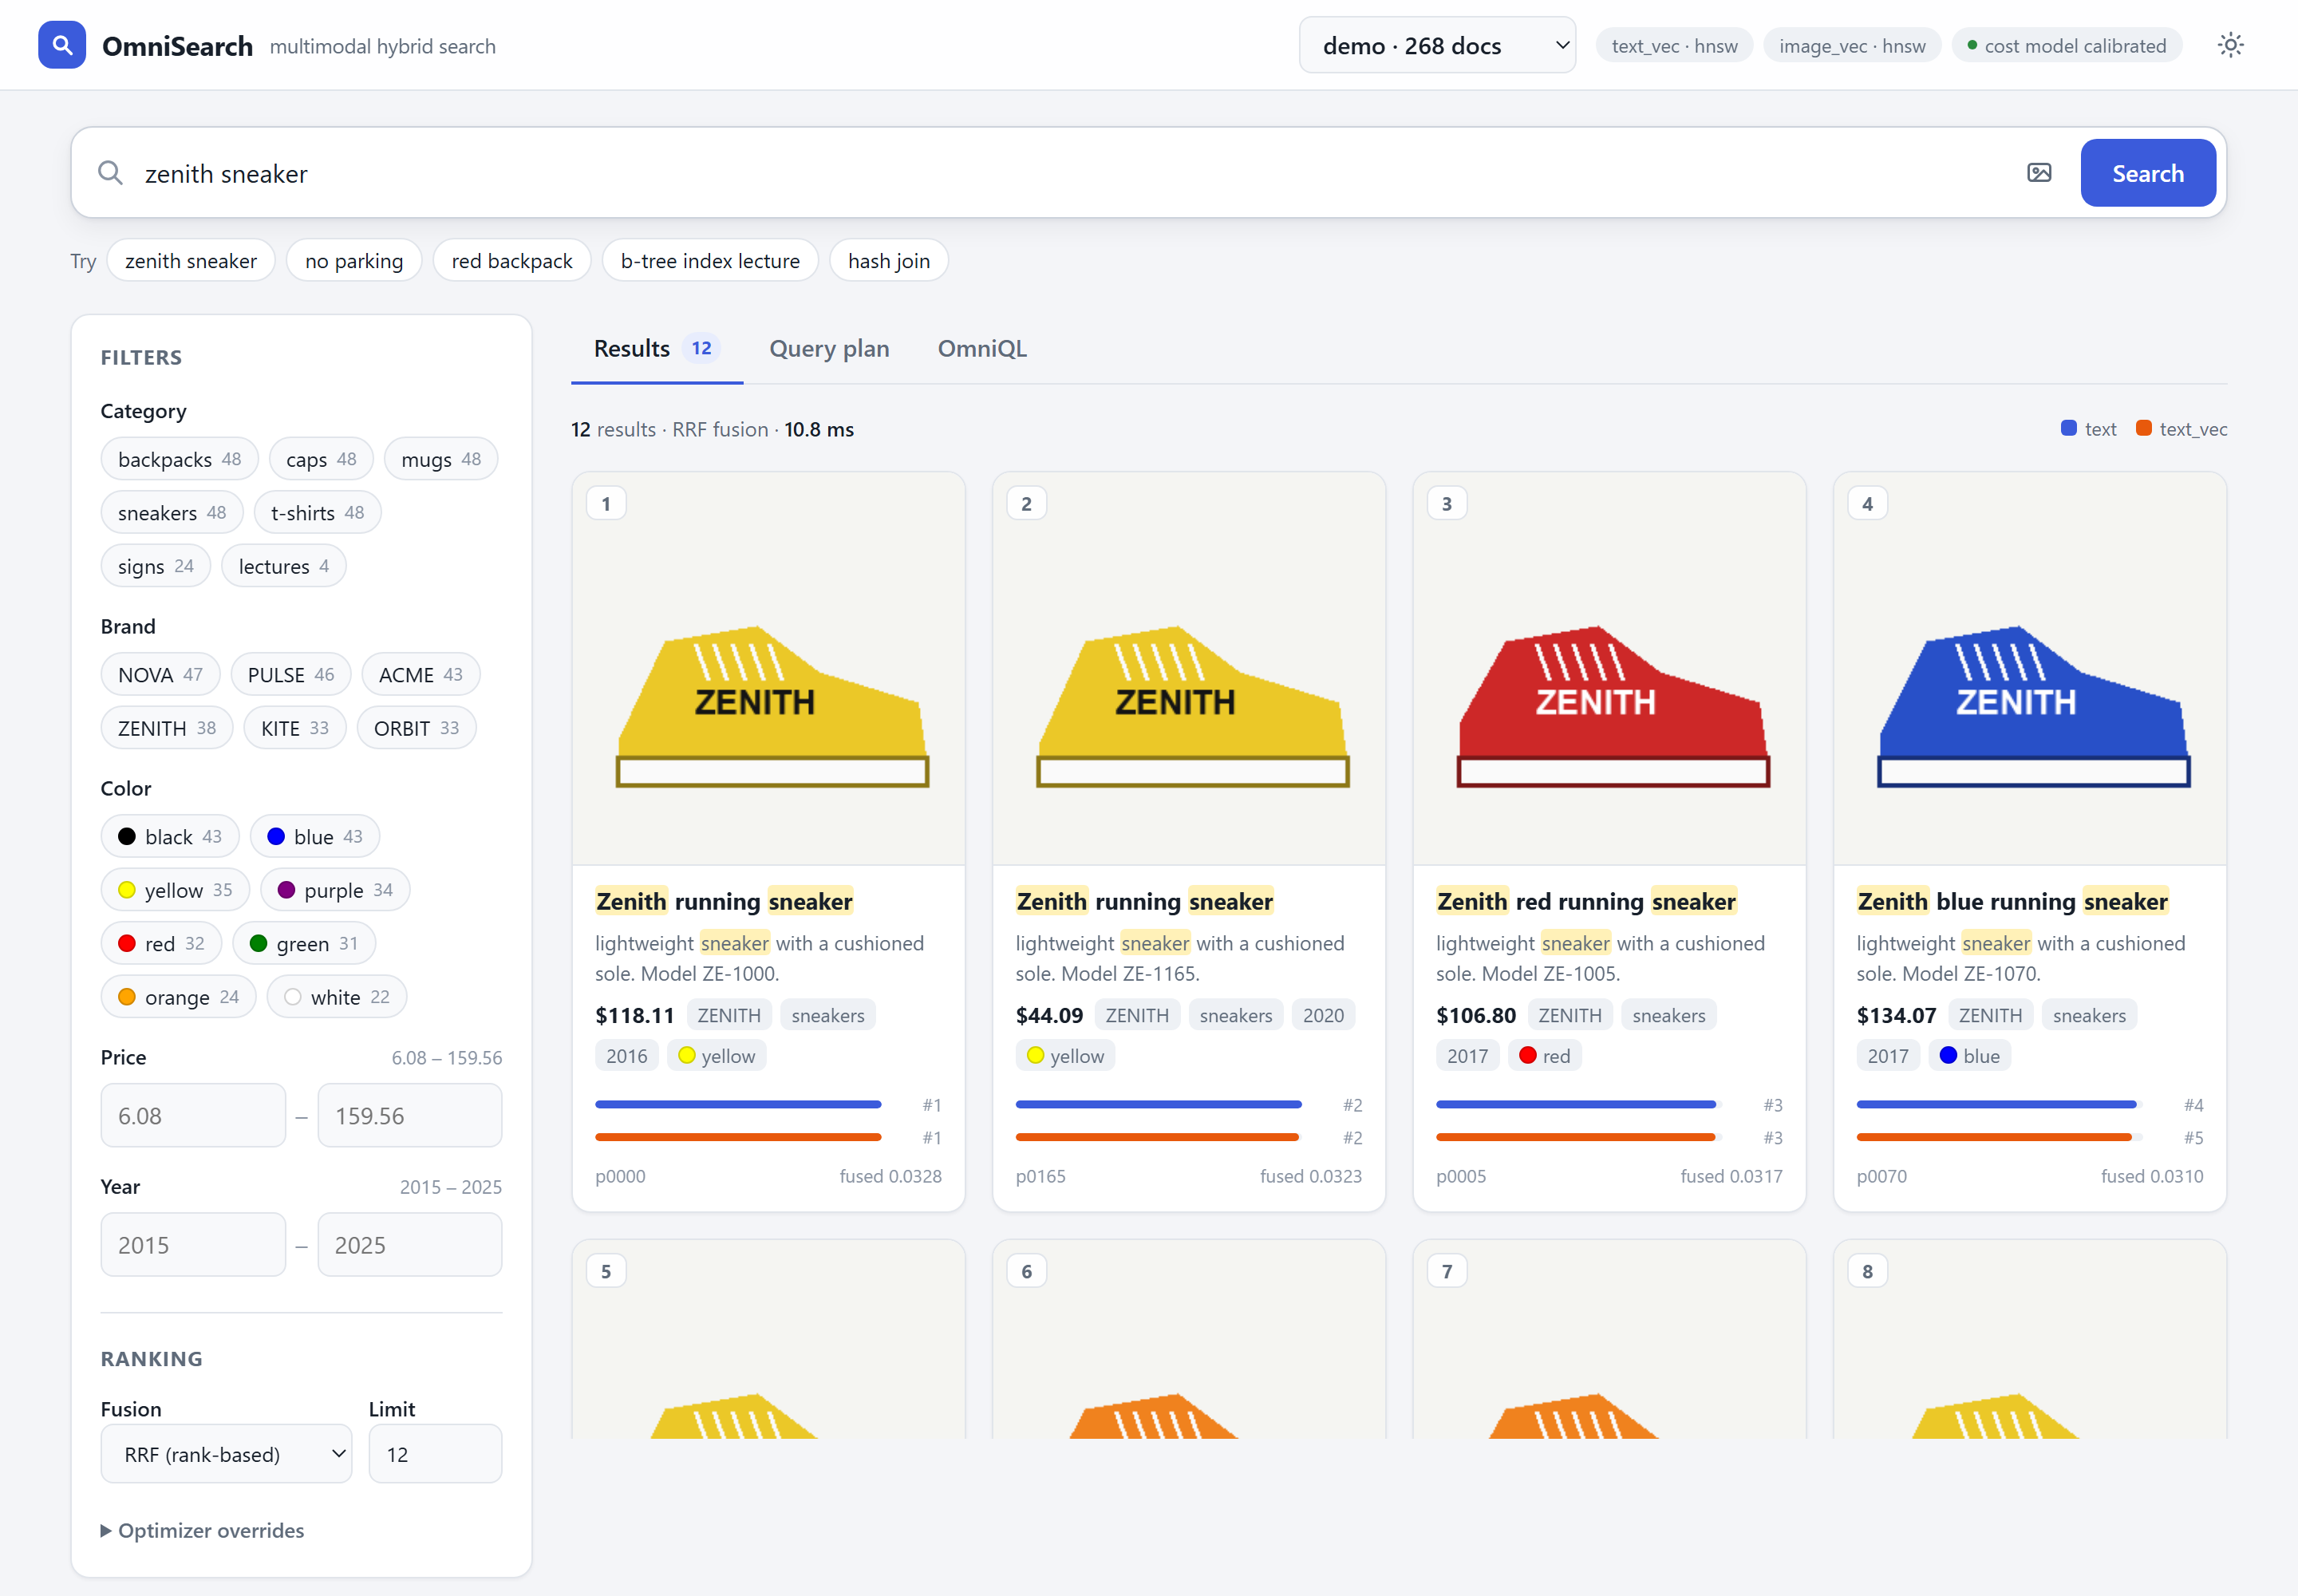
\includegraphics[width=0.86\linewidth]{ui-results.png}\\[4pt]
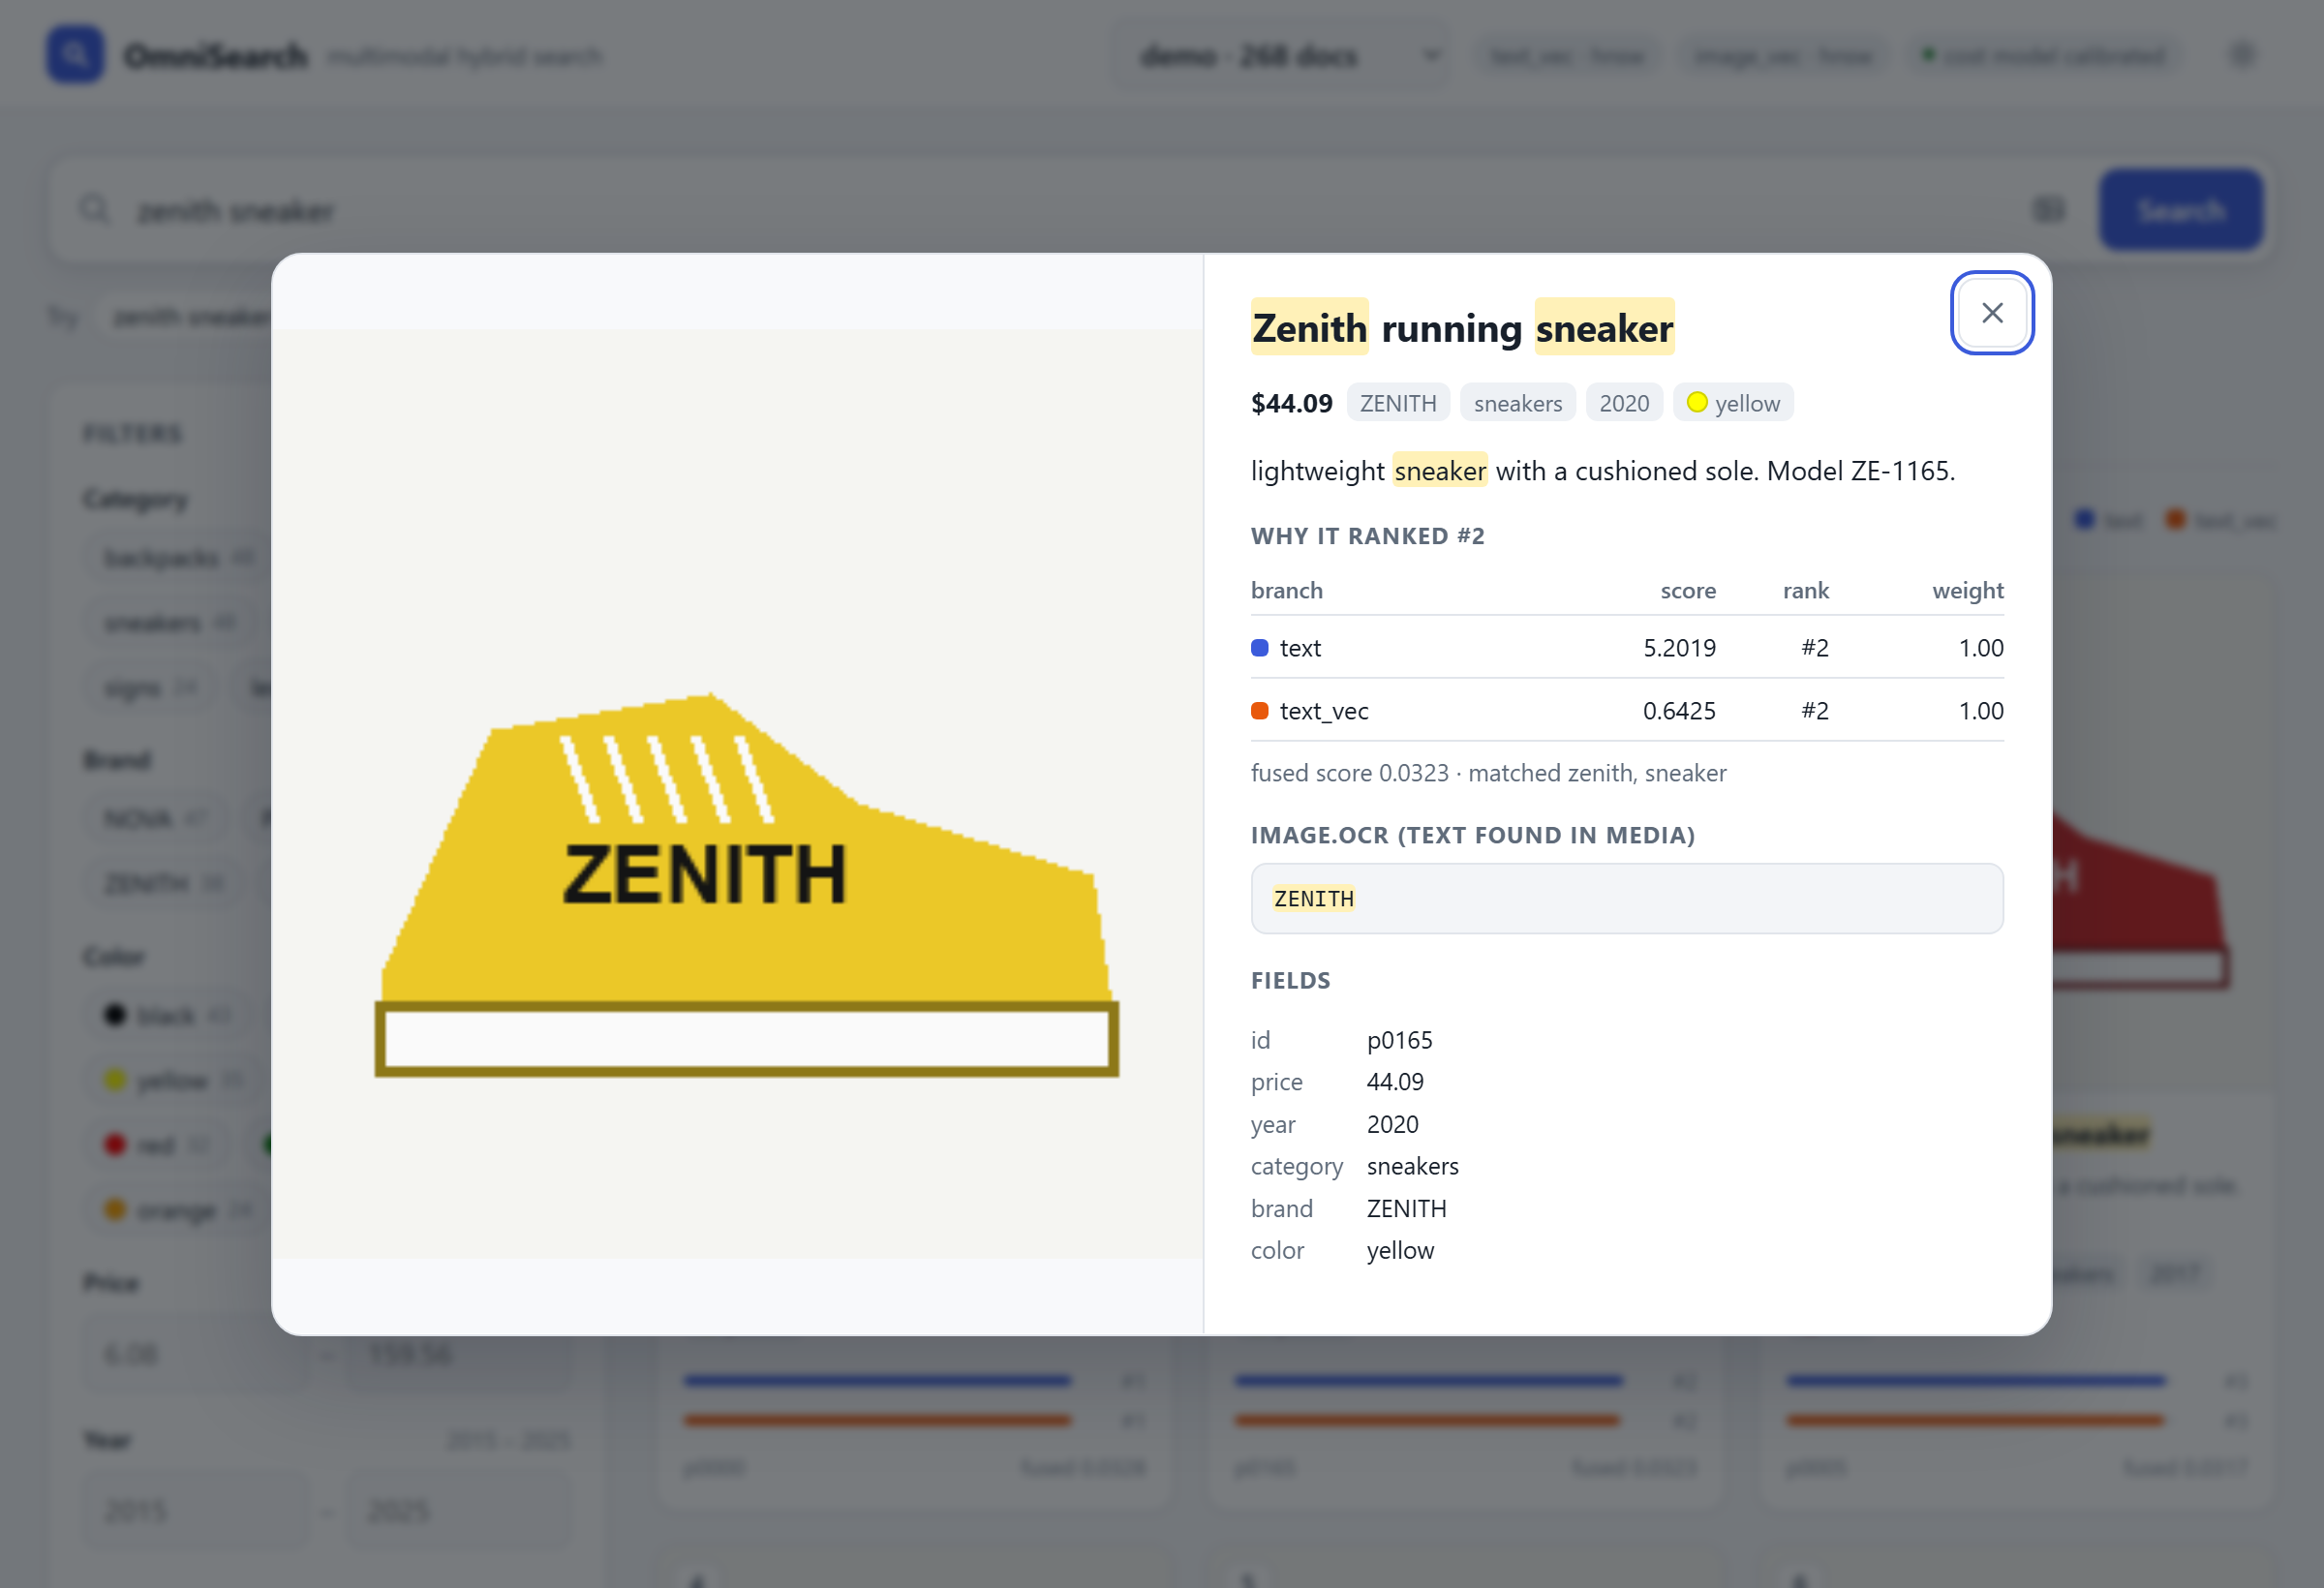
\includegraphics[width=0.43\linewidth]{ui-detail.png}\hspace{0.02\linewidth}%
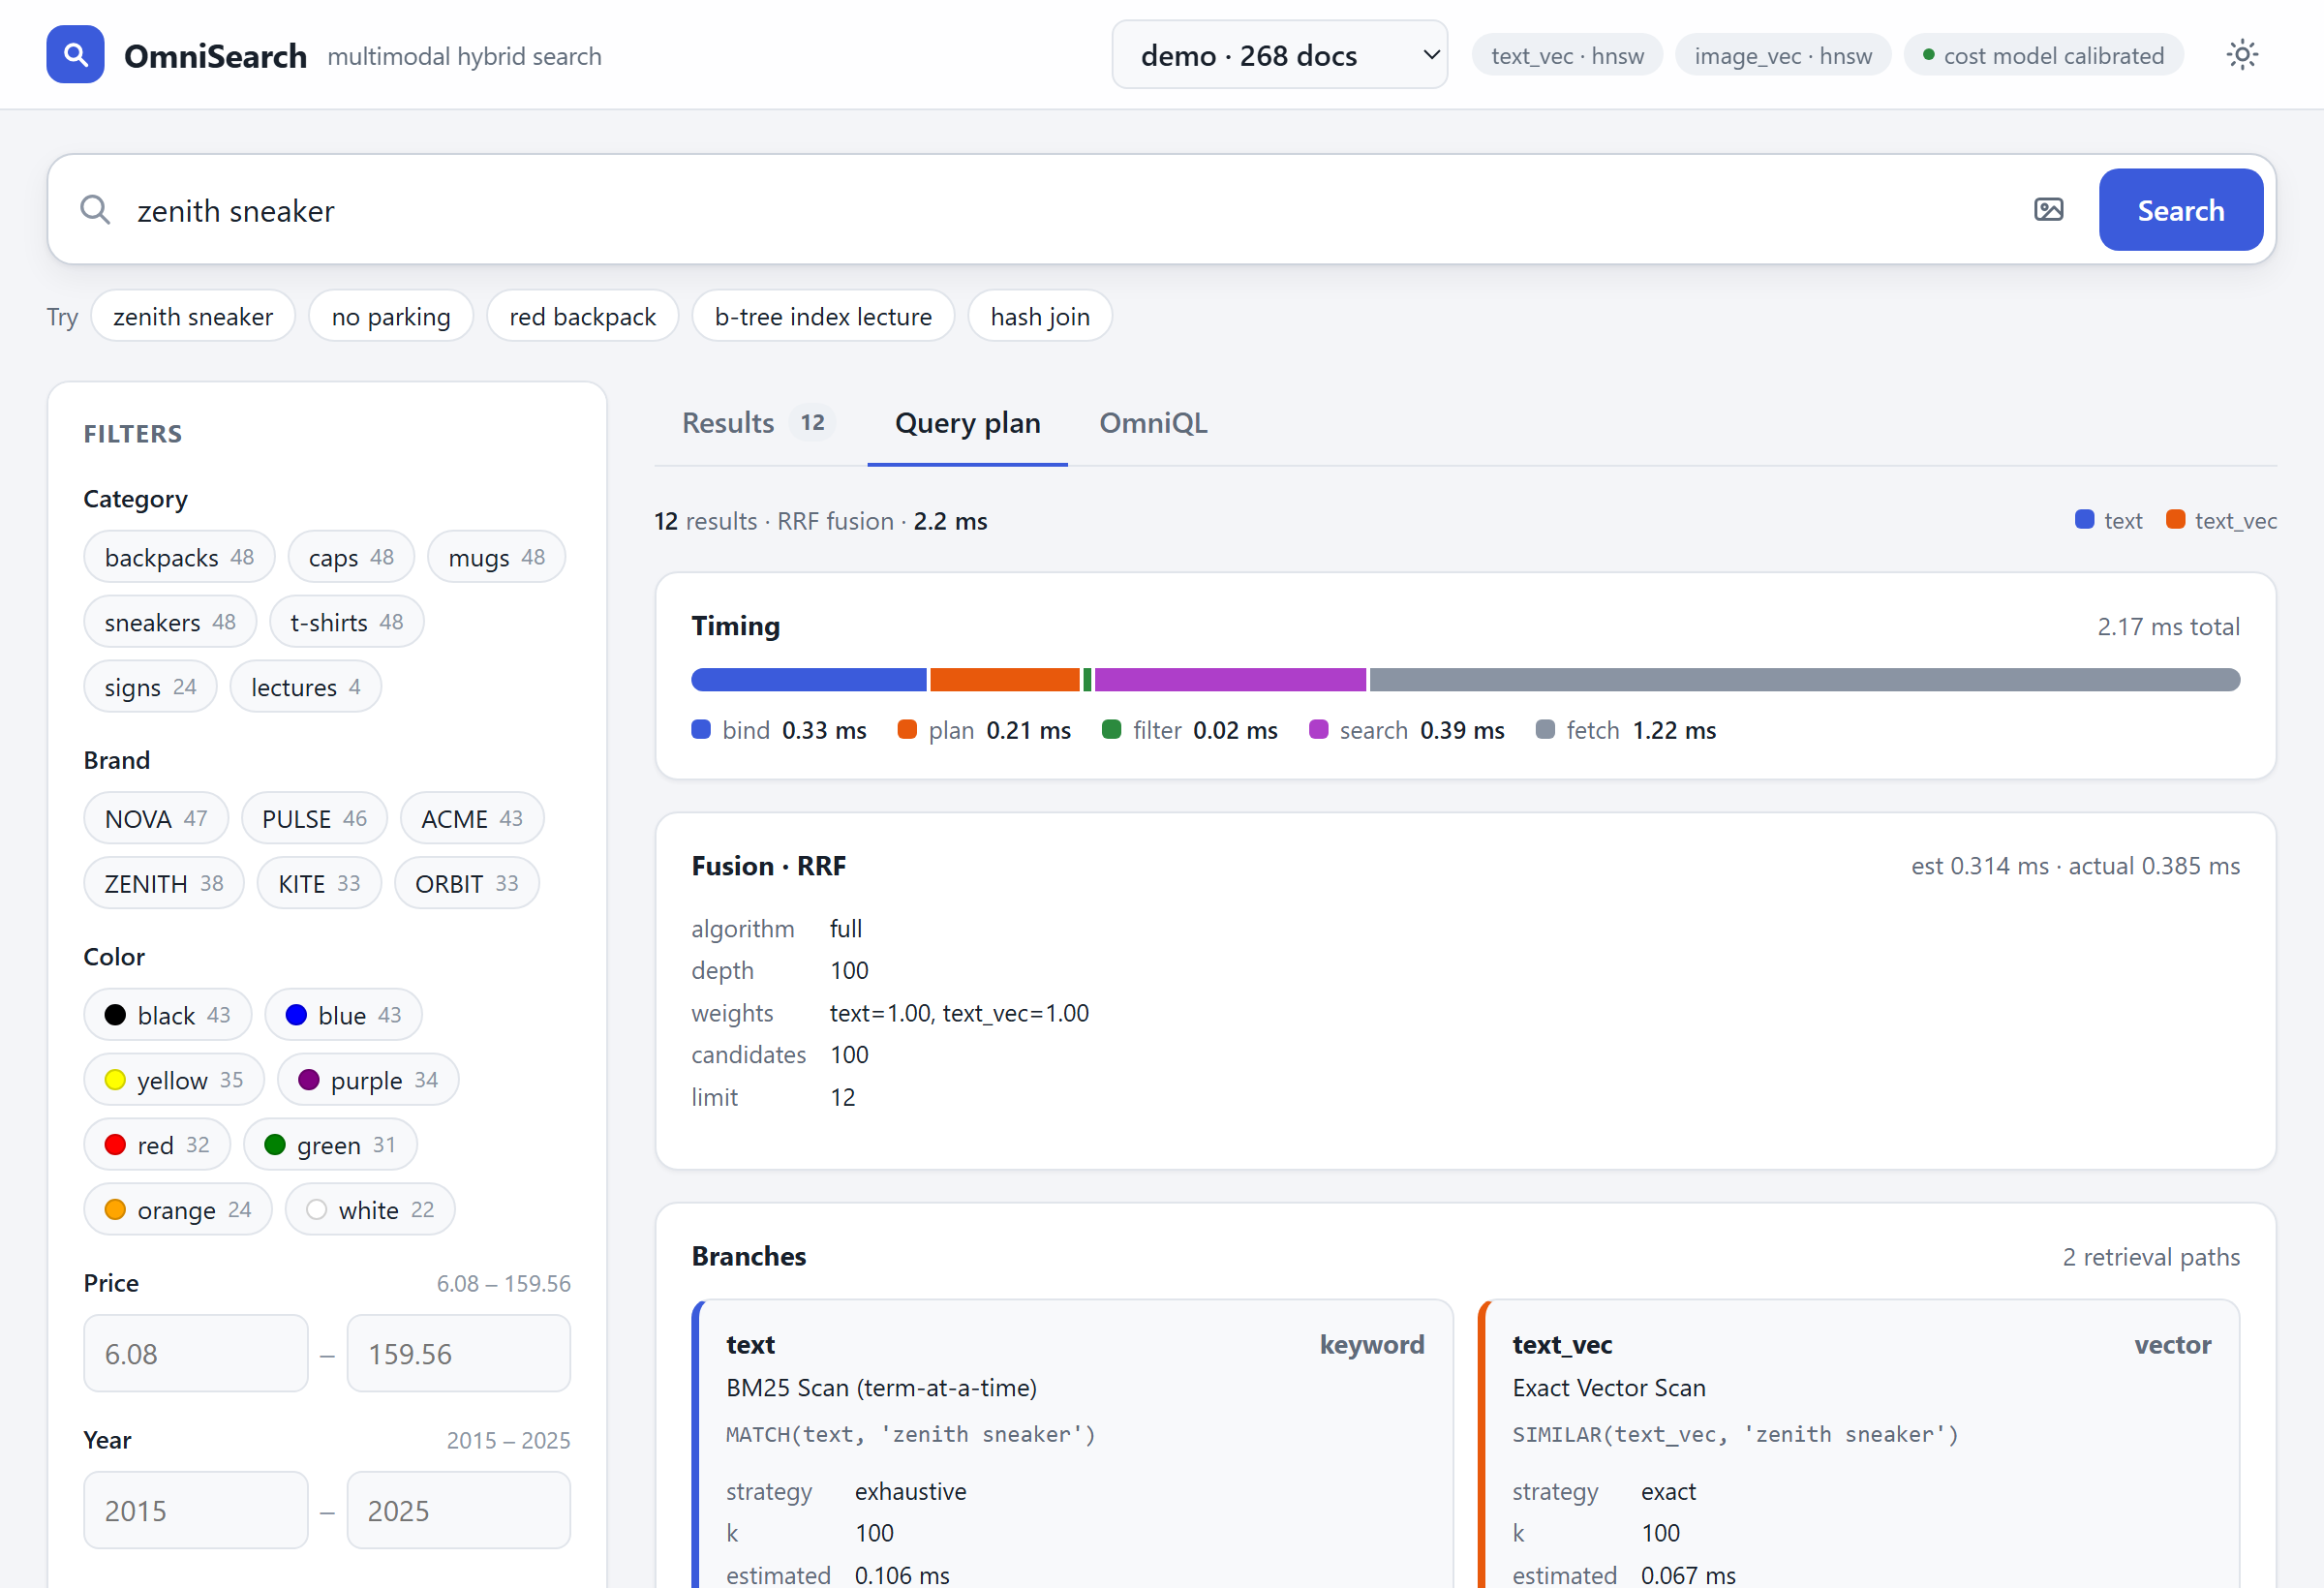
\includegraphics[width=0.43\linewidth]{ui-plan.png}
\caption{Web UI. Top: hybrid results for \emph{``zenith sneaker''}, with matched terms highlighted and
per-branch score bars (keyword in blue, vector in orange). Bottom left: the detail view explaining a
result's rank and showing the text OCR found in the image. Bottom right: the query-plan viewer with
the timing breakdown, the fusion operator and each branch's estimated vs.\ actual cost and rejected
alternatives.}
\label{fig:ui}
\end{figure}

% =====================================================================
\section{Experimental evaluation}
\label{sec:eval}

\subsection{Setup and datasets}

Systems experiments use synthetic data with \emph{controlled} structure. Isolating an index or optimizer
effect requires knowing the true selectivity, the true neighbours and the correlation between filter and
query, and real embeddings hide all three. Retrieval quality is measured on the demo collection, whose
ground truth is known by construction (\tab{tab:datasets}). Every benchmark writes JSON to
\code{results/}, and every table in this section is generated directly from those files, so no
number is copied by hand.

\begin{table}[h]
\centering\small
\begin{tabularx}{\linewidth}{lLl}
\toprule
Dataset & Construction & Used in \\
\midrule
Clustered vectors & $N = 20{,}000$ (50{,}000 for compression), $d = 128$, 64 Gaussian clusters on the unit sphere, cosine; 200 queries drawn near cluster centres; exact ground truth by brute force & \S\ref{sec:ann}, \S\ref{sec:opt-exp}, \S\ref{sec:quant} \\
Topic corpus & 50{,}000 documents, 30k-word Zipfian vocabulary; 35\% of each document's words from its cluster's topic vocabulary, so lexical and vector scores are correlated; 250 queries & \S\ref{sec:text-exp} \\
Top-$k$ corpus & 20{,}000 documents, topic text + $d=64$ clustered vectors; 2--3 ranked lists that are correlated (same topic) or independent & \S\ref{sec:topk-exp} \\
Attribute column & 200{,}000 rows; uniform \code{bucket} (exact selectivities), cluster-correlated \code{group}, log-normal (skewed) \code{price} & \S\ref{sec:filters-exp} \\
Scale & 10k, 25k and 50k documents with text, a 128-d vector and attributes & \S\ref{sec:scale} \\
Demo collection & 268 items: 240 rendered product photos (6 brands $\times$ 5 categories $\times$ 8 colours; brand printed on the product; a third of titles omit the colour), 24 street-sign photos (8 texts), 4 lecture videos (4 slides each) & \S\ref{sec:quality} \\
\bottomrule
\end{tabularx}
\caption{Datasets. All are generated reproducibly from fixed seeds.}
\label{tab:datasets}
\end{table}

\begin{table}[h]
\centering\small
\begin{tabular}{p{0.42\linewidth}p{0.5\linewidth}}
\toprule
Experiments & Environment \\
\midrule
Systems benchmarks (ANN, optimizer, top-$k$, text, filters, compression, scale) & Python 3.13.17, numpy 2.5.4, 4 CPUs (x86\_64), 2026-10-23 16:31 UTC \\
Demo retrieval quality & Python 3.11.9, numpy 2.4.6, 12 CPUs (AMD64), 2026-10-23 21:24 UTC \\
\bottomrule
\end{tabular}

\caption{Environments. Queries are single-threaded. FAISS~1.8 and SQLite FTS5 are the baselines.}
\label{tab:env}
\end{table}

% ---------------------------------------------------------------------
\subsection{ANN indexes: recall vs.\ latency}
\label{sec:ann}

\begin{figure}[H]
\centering
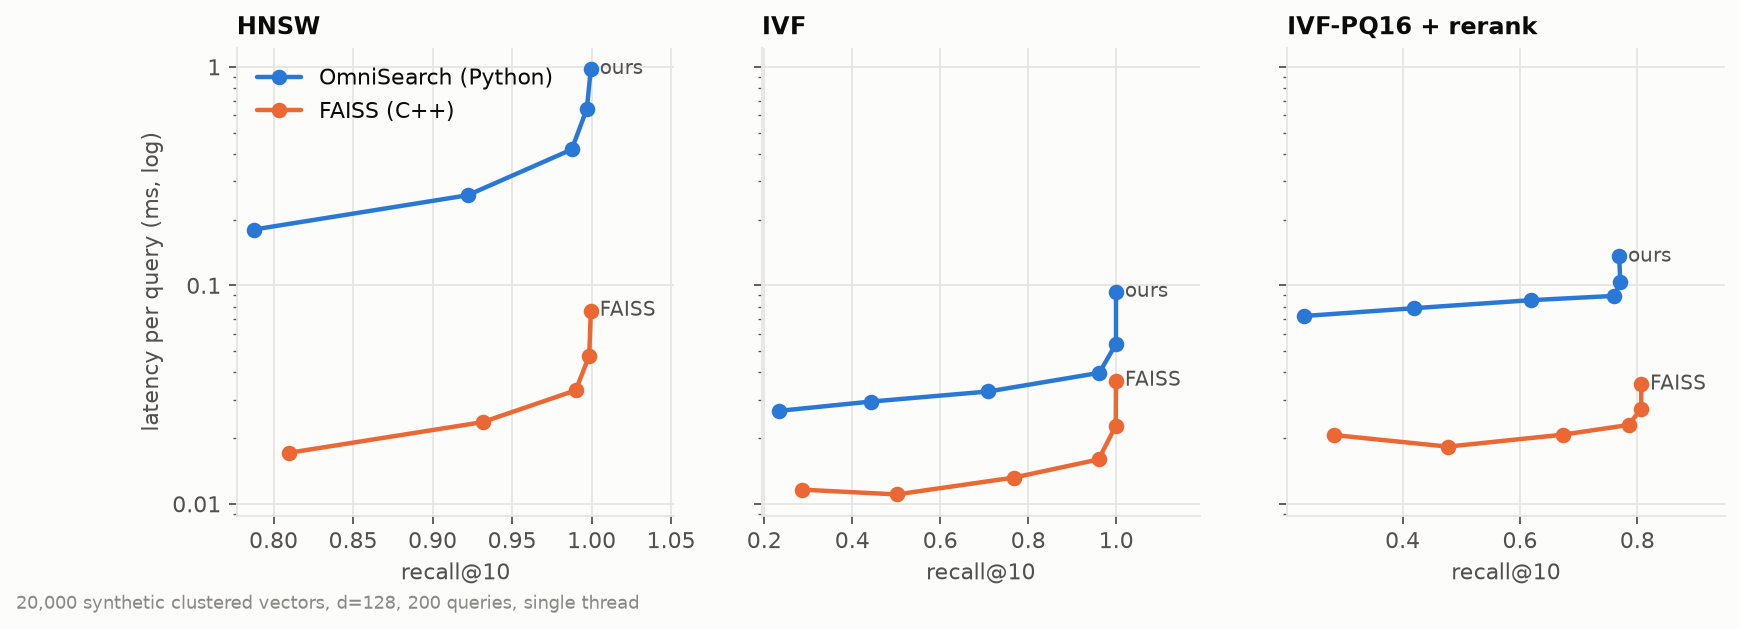
\includegraphics[width=\linewidth]{ann_recall_latency.png}
\caption{Recall@10 against query latency on 20{,}000 clustered 128-d vectors, sweeping $ef$ (HNSW) and
$nprobe$ (IVF).}
\label{fig:ann}
\end{figure}

\begin{table}[H]
\centering\small
\begin{tabular}{lrrr}
\toprule
Index & Build (s) & Best recall@10 & ms at recall $\geq$ 0.95 \\
\midrule
HNSW (ours) & 22.30 & 1.000 & 0.419 \\
IVF (ours) & 2.51 & 1.000 & 0.040 \\
IVF-PQ16 (ours) & 7.46 & 0.771 & -- \\
Exact scan (ours) & 0.01 & 1.000 & 0.147 \\
FAISS HNSW & 1.38 & 1.000 & 0.033 \\
FAISS IVF & 0.82 & 1.000 & 0.016 \\
FAISS IVF-PQ & 1.69 & 0.807 & -- \\
\bottomrule
\end{tabular}

\caption{Build time, best recall and the fastest setting that reaches recall $\geq 0.95$.}
\label{tab:ann}
\end{table}

Our HNSW reaches recall 1.00 but costs 0.42\,ms per query against 0.033\,ms for FAISS's C++
implementation ($\approx$13$\times$). Our IVF is within 2.5$\times$ of FAISS, because its inner loop
is a vectorised partition scan rather than interpreted graph traversal. At 20k vectors a vectorised
exact scan (0.15\,ms) still beats our HNSW. The calibrated cost model knows this and chooses the exact
scan for unfiltered queries at this size (\tab{tab:optimizer}, last row, is the crossover). IVF-PQ16
plateaus at recall 0.77; product quantization is weak on these isotropic synthetic vectors
(\sect{sec:quant}).

% ---------------------------------------------------------------------
\subsection{The cost-based optimizer for filtered vector search}
\label{sec:opt-exp}

\begin{figure}[H]
\centering
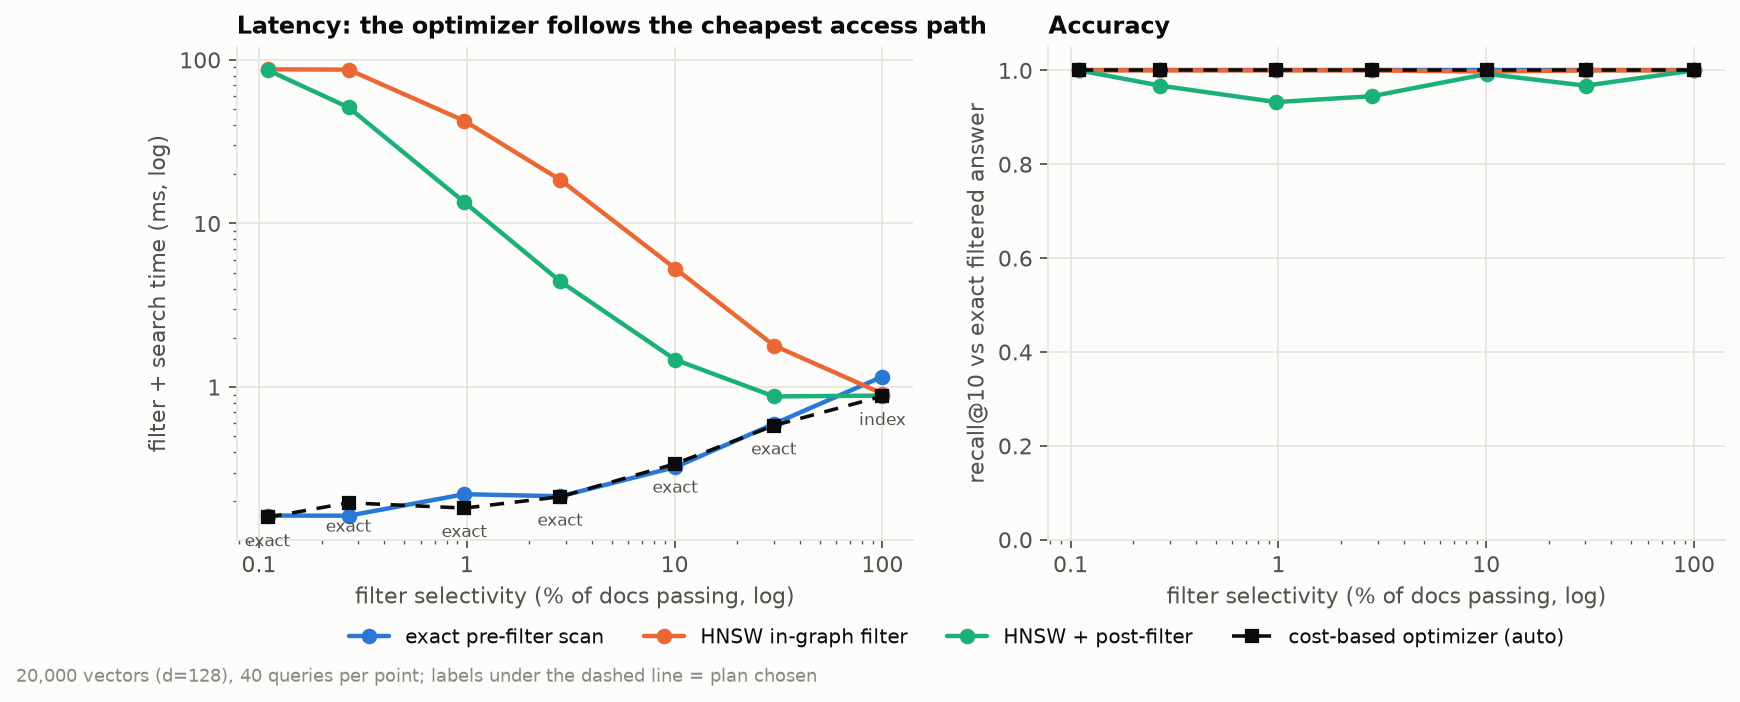
\includegraphics[width=\linewidth]{optimizer_selectivity.png}
\caption{Latency (left) and recall (right) of each filtered access path as filter selectivity varies,
and the plan chosen by the optimizer (dashed).}
\label{fig:optimizer}
\end{figure}

\begin{table}[H]
\centering\small
\begin{tabular}{rrrrrl}
\toprule
Selectivity & Exact & In-graph & Post-filter (rec.) & Optimizer (rec.) & Chosen \\
\midrule
0.11\% & 0.16 & 87.53 & 86.71 (1.00) & \textbf{0.16} (1.00) & exact \\
0.27\% & 0.16 & 87.16 & 51.21 (0.97) & \textbf{0.20} (1.00) & exact \\
0.97\% & 0.22 & 42.37 & 13.48 (0.93) & \textbf{0.18} (1.00) & exact \\
2.82\% & 0.22 & 18.47 & 4.42 (0.95) & \textbf{0.21} (1.00) & exact \\
10.08\% & 0.32 & 5.30 & 1.47 (0.99) & \textbf{0.34} (1.00) & exact \\
30.09\% & 0.60 & 1.79 & 0.88 (0.97) & \textbf{0.58} (1.00) & exact \\
100.00\% & 1.16 & 0.91 & 0.89 (1.00) & \textbf{0.88} (1.00) & index \\
\bottomrule
\end{tabular}

\caption{Mean latency (ms) and recall@10 per access path. ``Optimizer'' is the plan chosen by the
cost model.}
\label{tab:optimizer}
\end{table}

\begin{table}[H]
\centering\small
\begin{tabular}{lrrrr}
\toprule
Filter & Exact & In-graph & Post-filter & Optimizer \\
\midrule
correlated & 0.16 (1.00) & 1.26 (1.00) & 8.21 (1.00) & 0.15 (1.00) \\
anti-correlated & 0.16 (1.00) & 29.12 (1.00) & 8.82 (0.82) & 0.20 (1.00) \\
\bottomrule
\end{tabular}

\caption{Same selectivity, different correlation: the filter selects documents in the query's own
cluster (correlated) or away from it (anti-correlated). Latency in ms (recall@10).}
\label{tab:correlation}
\end{table}

\textbf{The optimizer tracks the lower envelope.} With a 0.1\% filter the pre-filtered exact scan takes
0.16\,ms, while HNSW with in-graph filtering takes 87.5\,ms ($540\times$ slower) because the beam must
expand on the order of $1/s$ nodes to find $ef$ allowed ones. Post-filtering is just as slow, because it
must over-fetch $1.5k/s$ results, and it also loses recall (0.93 at 1\%). The optimizer chooses the exact
scan up to 30\% selectivity and switches to HNSW only for the unfiltered query, with recall 1.00 at
every point (\fig{fig:optimizer}).

\textbf{Correlation matters as much as selectivity.} At equal selectivity, in-graph HNSW filtering costs
1.3\,ms when the allowed documents lie in the query's neighbourhood and 29\,ms when they lie away from
it; post-filter recall drops from 1.00 to 0.82 (\tab{tab:correlation}). An optimizer that assumes
independence cannot see this. It is the failure mode that motivates ACORN~\cite{acorn}, and here the
cost model avoids it by preferring the exact plan whenever the filtered set is small.

% ---------------------------------------------------------------------
\subsection{Top-\texorpdfstring{$k$}{k} fusion algorithms}
\label{sec:topk-exp}

\begin{figure}[H]
\centering
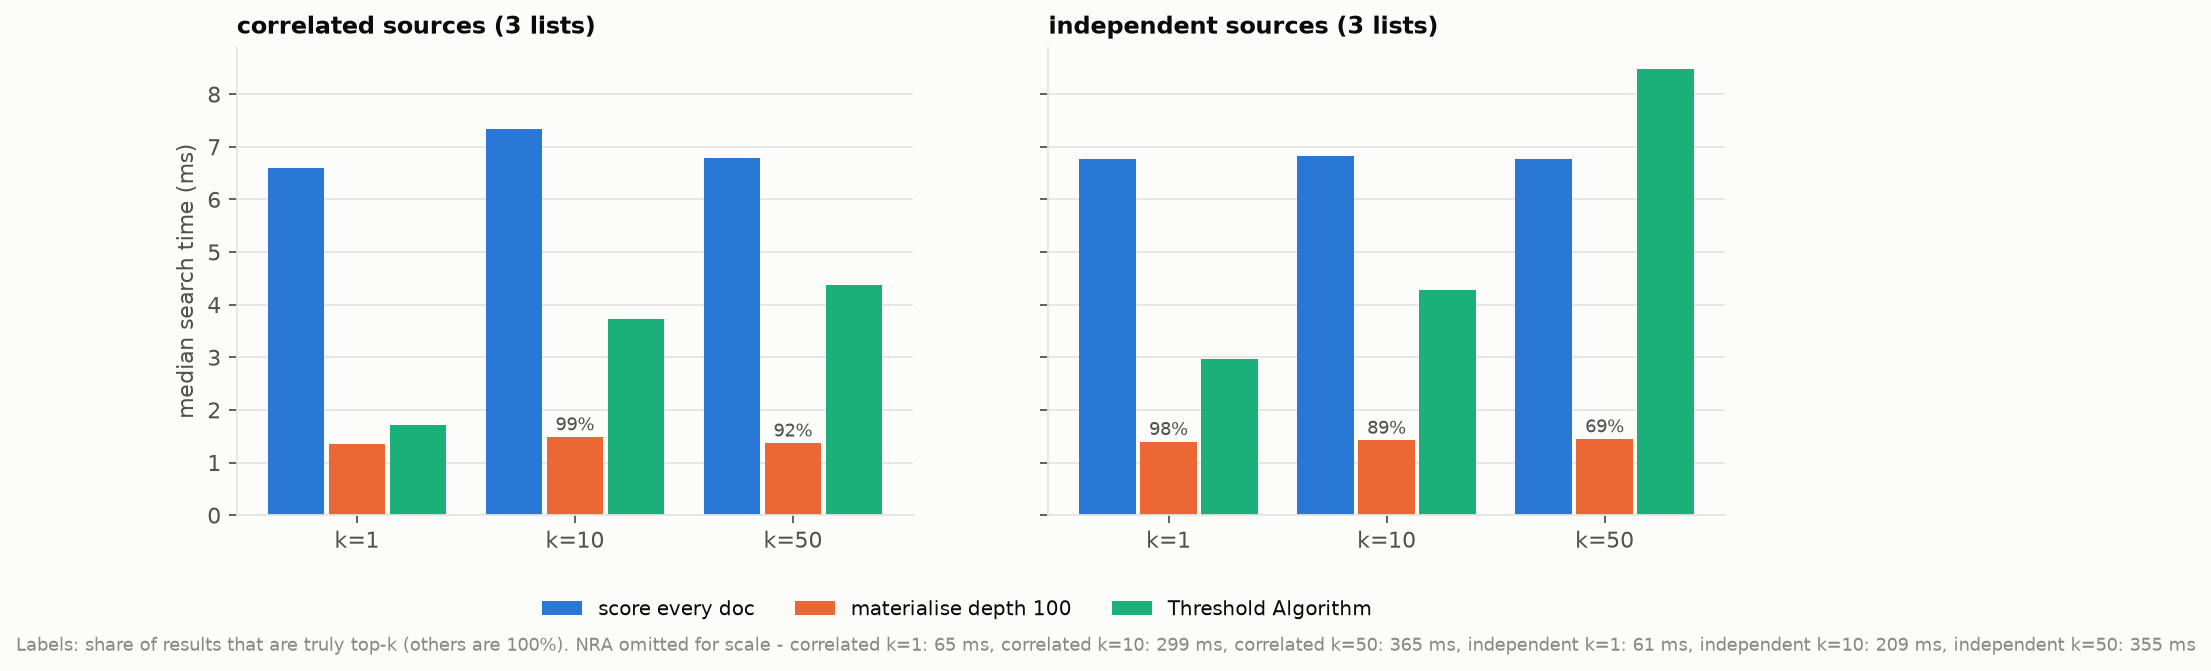
\includegraphics[width=\linewidth]{topk_algorithms.png}
\caption{Weighted fusion of $m$ ranked lists: latency, accesses and exactness of each top-$k$
algorithm.}
\label{fig:topk}
\end{figure}

\begin{table}[H]
\centering\small
\begin{tabular}{lrrrrrrr}
\toprule
Lists & $m$ & $k$ & Exhaustive & Merge@100 & TA & TA accesses & NRA \\
\midrule
correlated & 2 & 1 & 3.89 & 0.73 (100\%) & 0.32 (100\%) & 19+18 & 1.09 (100\%) \\
correlated & 2 & 10 & 3.81 & 0.72 (100\%) & 0.60 (100\%) & 59+57 & 2.91 (100\%) \\
correlated & 2 & 50 & 3.86 & 0.74 (100\%) & 1.23 (100\%) & 190+170 & 6.65 (100\%) \\
correlated & 3 & 1 & 6.60 & 1.36 (100\%) & 1.71 (100\%) & 159+302 & 65.23 (100\%) \\
correlated & 3 & 10 & 7.34 & 1.49 (99\%) & 3.73 (100\%) & 405+733 & 299.33 (100\%) \\
correlated & 3 & 50 & 6.79 & 1.37 (92\%) & 4.37 (100\%) & 609+1098 & 365.24 (100\%) \\
\midrule
independent & 2 & 1 & 4.16 & 0.76 (100\%) & 0.90 (100\%) & 131+131 & 28.03 (100\%) \\
independent & 2 & 10 & 3.90 & 0.78 (100\%) & 1.71 (100\%) & 245+245 & 45.57 (100\%) \\
independent & 2 & 50 & 3.94 & 0.78 (99\%) & 1.64 (100\%) & 274+274 & 51.23 (100\%) \\
independent & 3 & 1 & 6.77 & 1.40 (98\%) & 2.97 (100\%) & 367+729 & 61.02 (100\%) \\
independent & 3 & 10 & 6.82 & 1.42 (89\%) & 4.29 (100\%) & 505+1002 & 209.41 (100\%) \\
independent & 3 & 50 & 6.77 & 1.45 (69\%) & 8.47 (100\%) & 951+1876 & 355.09 (100\%) \\
\bottomrule
\end{tabular}

\caption{Latency in ms; in parentheses, the fraction of the true top-$k$ returned. ``Merge@100''
materialises each list to depth 100 and merges. ``TA accesses'' counts sorted + random accesses.}
\label{tab:topk}
\end{table}

\textbf{TA is exact and stops early.} With two correlated lists, TA returns the exact top-1 after only
19 sorted and 18 random accesses, in 0.32\,ms against 3.89\,ms for scoring every document
(12$\times$). Fixed-depth merge is fast, but it is \emph{wrong} exactly where fusion matters most: with
three independent lists it returns only 69\% of the true top-50, because true top-50 documents rank
below 100 in some list. TA stays at 100\% in every setting. \textbf{NRA} is exact too, but it is the
slowest here. It avoids random access, the right trade-off when random access is expensive (a remote
service), whereas here a random access is a cheap in-memory lookup. Its per-candidate bound
bookkeeping also runs in the interpreter.

% ---------------------------------------------------------------------
\subsection{Keyword index}
\label{sec:text-exp}

\begin{figure}[H]
\centering
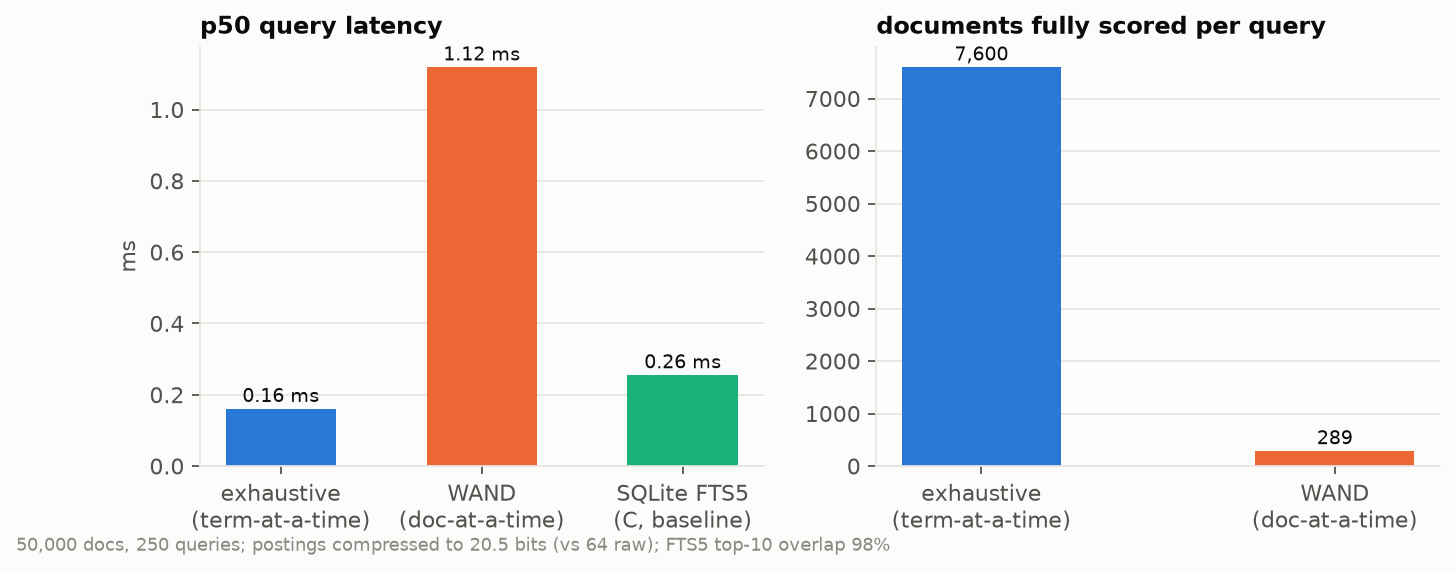
\includegraphics[width=0.92\linewidth]{keyword_index.png}
\caption{Posting-list compression and BM25 query latency (exhaustive vs.\ WAND vs.\ SQLite FTS5).}
\label{fig:text}
\end{figure}

\begin{table}[H]
\centering\small
\begin{tabular}{lr}
\toprule
Metric & Value \\
\midrule
Documents / distinct terms & 50,000 / 29,083 \\
Postings & 1,057,314 \\
Index size, compressed vs raw & 2.71 MB vs 8.46 MB \\
Bits per posting & 20.5 \\
Vectorised VByte decode & 46 M integers/s \\
BM25 p50 latency: exhaustive / WAND & 0.16 ms / 1.12 ms \\
Documents fully scored: exhaustive / WAND & 7,600 / 289 \\
SQLite FTS5 p50 latency & 0.26 ms \\
Top-10 overlap with FTS5 & 98\% \\
\bottomrule
\end{tabular}

\caption{Inverted index on the 50k-document topic corpus.}
\label{tab:text}
\end{table}

Gap + VByte coding stores a posting in 20.5 bits, 3.1$\times$ smaller than raw 32-bit pairs. Our BM25
top-10 agrees 98\% with SQLite FTS5's \code{bm25()} ranking, and the median latency is lower (0.16 vs.\
0.26\,ms). WAND scores 26$\times$ fewer documents (289 vs.\ 7{,}600), yet it is \emph{slower} in Python
(1.12\,ms). Its savings are in work, but each pivot step is interpreted, while exhaustive scoring is one
vectorised pass per term. The cost model includes a per-step WAND cost, so it chooses WAND only for
queries with very long posting lists.

% ---------------------------------------------------------------------
\subsection{Attribute filters and selectivity estimation}
\label{sec:filters-exp}

\begin{figure}[H]
\centering
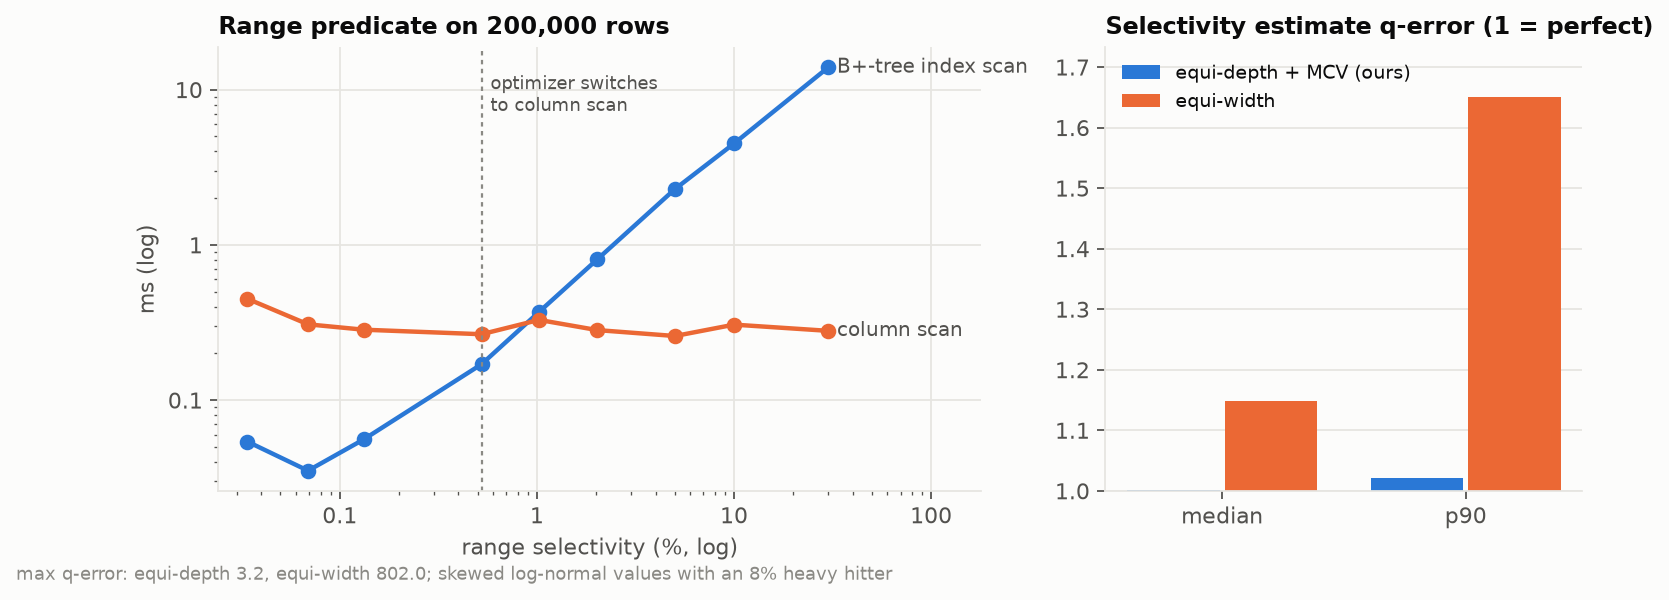
\includegraphics[width=\linewidth]{filters.png}
\caption{Left: B$^+$-tree range scan vs.\ vectorised column scan on 200k rows. Right: selectivity
estimation error of equi-depth + MCV vs.\ equi-width histograms on a skewed column.}
\label{fig:filters}
\end{figure}

\begin{table}[H]
\centering\small
\begin{tabular}{rrrl}
\toprule
Selectivity & B+-tree (ms) & Column scan (ms) & Optimizer choice \\
\midrule
0.034\% & 0.054 & 0.450 & B+-tree \\
0.069\% & 0.035 & 0.308 & B+-tree \\
0.132\% & 0.056 & 0.284 & B+-tree \\
0.524\% & 0.170 & 0.266 & column scan \\
1.025\% & 0.370 & 0.329 & column scan \\
2.023\% & 0.806 & 0.283 & column scan \\
5.020\% & 2.291 & 0.259 & column scan \\
10.018\% & 4.504 & 0.306 & column scan \\
30.020\% & 13.895 & 0.279 & column scan \\
\bottomrule
\end{tabular}
\\[8pt]
\begin{tabular}{lrrr}
\toprule
Statistics & Median & p90 & Max \\
\midrule
Equi-depth + MCV (ours) & 1.00 & 1.02 & 3.2 \\
Equi-width & 1.15 & 1.65 & 802.0 \\
\bottomrule
\end{tabular}

\caption{Top: B$^+$-tree vs.\ column scan latency per range selectivity and the optimizer's choice.
Bottom: q-error of range-selectivity estimates, $\max(\hat{s}/s,\, s/\hat{s})$, on the skewed column.}
\label{tab:filters}
\end{table}

The B$^+$-tree wins below about 0.5\% selectivity. Above that, gathering rows one by one from the tree
loses to a vectorised scan of the whole column, which costs a near-constant 0.3\,ms. The optimizer
switches at exactly that point. Equi-depth histograms with most-common values estimate range
selectivity with a median q-error of 1.00 and a maximum of 3.2; equi-width histograms reach 802 on the
skewed price column. A wrong estimate of that size would send the vector optimizer to the wrong plan in
\tab{tab:optimizer}.

% ---------------------------------------------------------------------
\subsection{Vector compression}
\label{sec:quant}

\begin{figure}[H]
\centering
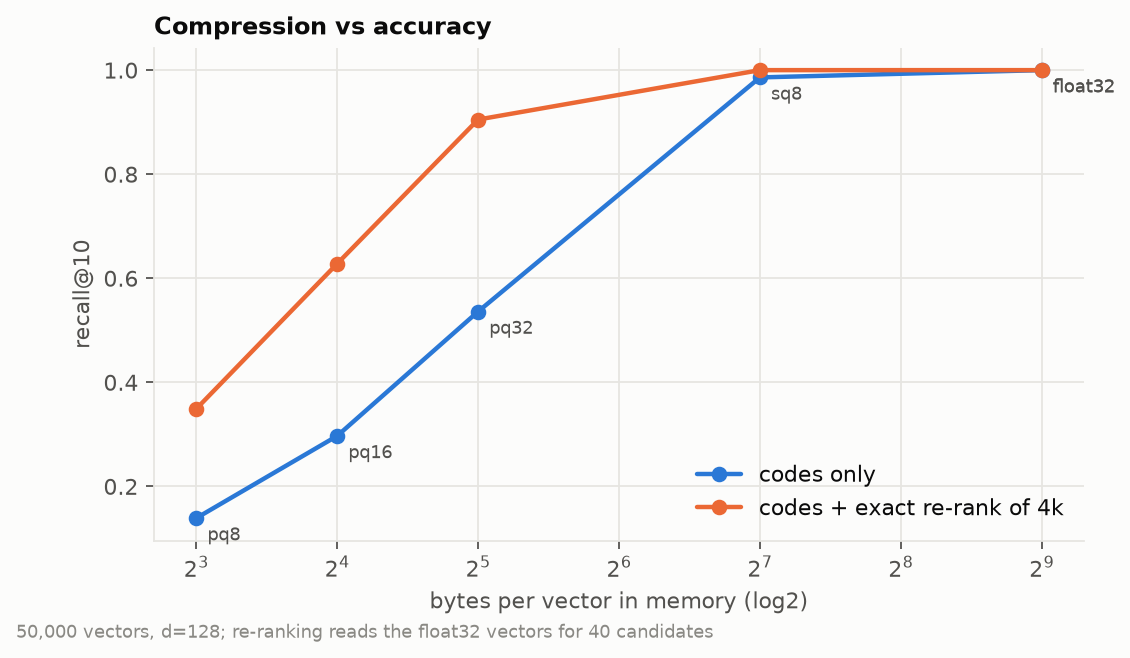
\includegraphics[width=0.72\linewidth]{quantization.png}
\caption{Memory per vector against recall@10 (50{,}000 vectors, $d=128$), with and without exact
re-ranking.}
\label{fig:quant}
\end{figure}

\begin{table}[H]
\centering\small
\begin{tabular}{lrrrr}
\toprule
Codes & Re-rank & Bytes/vector & Recall@10 & ms/query \\
\midrule
float32 & -- & 512 & 1.000 & 0.71 \\
SQ8 & -- & 128 & 0.986 & 1.77 \\
SQ8 & 4 & 128 & 1.000 & 1.85 \\
PQ32 & -- & 32 & 0.536 & 4.67 \\
PQ32 & 4 & 32 & 0.905 & 4.54 \\
PQ16 & -- & 16 & 0.297 & 2.02 \\
PQ16 & 4 & 16 & 0.628 & 1.91 \\
PQ8 & -- & 8 & 0.139 & 1.06 \\
PQ8 & 4 & 8 & 0.349 & 1.07 \\
\bottomrule
\end{tabular}

\caption{Compression vs.\ recall. Re-rank $r$ = exact re-scoring of the top $r\cdot k$ candidates.}
\label{tab:quant}
\end{table}

SQ8 cuts memory 4$\times$ at recall 0.986, and 1.000 with re-ranking. PQ32 (16$\times$ smaller) needs
re-ranking to reach 0.905, and PQ16 and PQ8 lose most neighbours. These synthetic vectors are isotropic
within each cluster, which is the worst case for product quantization: there is no low-dimensional
structure for the sub-codebooks to capture. Real CLIP embeddings are far more compressible.

% ---------------------------------------------------------------------
\subsection{Scale}
\label{sec:scale}

\begin{figure}[H]
\centering
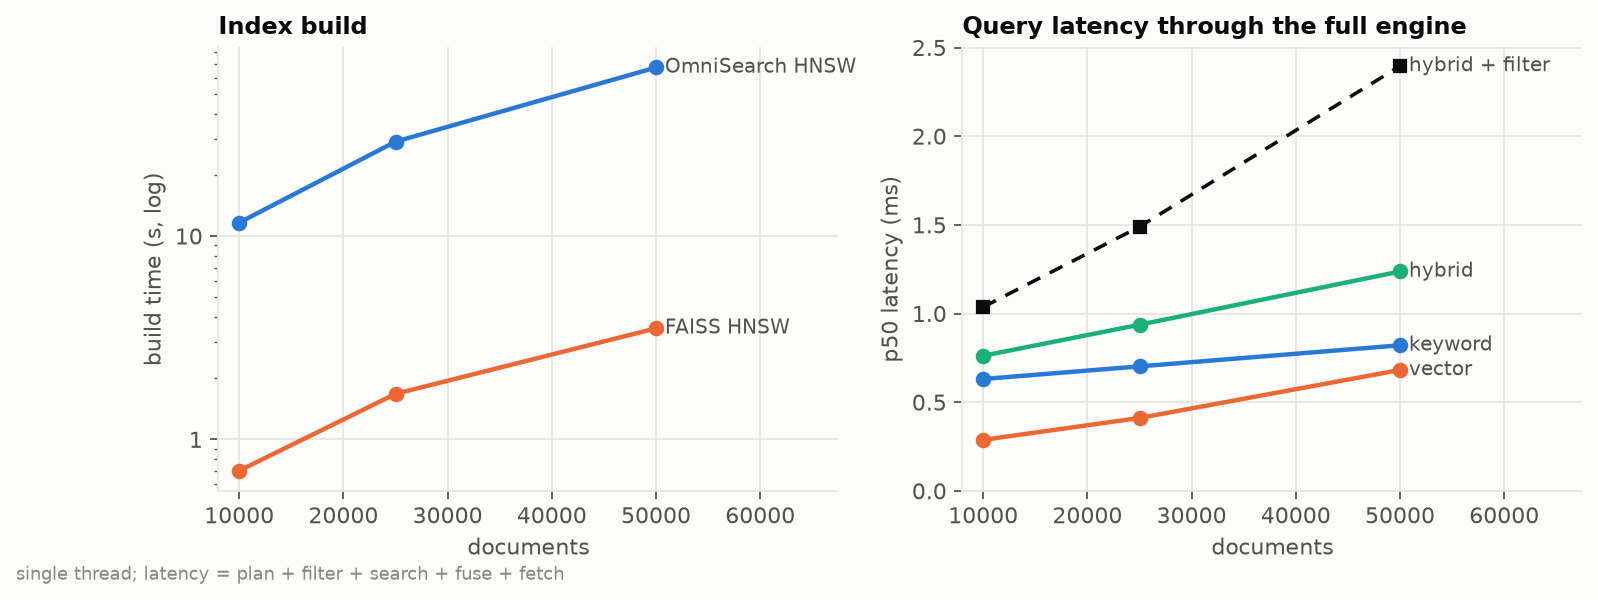
\includegraphics[width=\linewidth]{scale.png}
\caption{Build time, disk footprint and p50 query latency from 10k to 50k documents.}
\label{fig:scale}
\end{figure}

\begin{table}[H]
\centering\small
\begin{tabular}{rrrrrrrrr}
\toprule
Docs & Ingest (s) & HNSW (s) & FAISS (s) & Disk (MB) & Keyword & Vector & Hybrid & +Filter \\
\midrule
10,000 & 0.3 & 11.6 & 0.70 & 10.1 & 0.63 & 0.29 & 0.76 & 1.04 \\
25,000 & 0.8 & 29.1 & 1.67 & 29.0 & 0.70 & 0.41 & 0.94 & 1.49 \\
50,000 & 1.7 & 67.5 & 3.52 & 53.3 & 0.82 & 0.68 & 1.24 & 2.40 \\
\bottomrule
\end{tabular}

\caption{Scaling. Build times in seconds; the last four columns are p50 query latency in ms.}
\label{tab:scale}
\end{table}

Ingest and on-disk size grow linearly (53\,MB at 50k documents). HNSW construction dominates build
time: 67.5\,s against 3.5\,s for FAISS, with the same interpreted-graph overhead seen in
\sect{sec:ann}. Query latency grows sub-linearly: a hybrid query takes 1.24\,ms at 50k documents and
2.40\,ms with a filter.

% ---------------------------------------------------------------------
\subsection{Retrieval quality on the demo collection}
\label{sec:quality}

The systems experiments measure speed and exactness. This experiment measures \emph{which retrieval path
finds the right documents}. The collection is the 268-item demo collection built with the offline
\emph{classic} profile. Text is indexed from titles, descriptions and the OCR of every image and video
keyframe (RapidOCR, PP-OCRv4). The vector side is \code{text\_vec}, a 512-d hashed character-$n$-gram
embedding of the same text. Relevance labels come from the data generator, never from the engine. Five
query sets each probe a different path:
\begin{itemize}
  \item \textbf{brand+category} (\emph{``zenith sneaker''}): words present in titles;
  \item \textbf{colour+category} (\emph{``red mug''}): a third of the titles omit the colour, which
        only the pixels show;
  \item \textbf{typos} (\emph{``zenth sneker''}): the middle letter of every word of 4+ letters is
        deleted;
  \item \textbf{sign text (OCR)} (\emph{``no parking''}): the text exists only inside the photo;
  \item \textbf{lecture (OCR)} (\emph{``extendible hashing''}): the phrase appears only on a slide
        inside the video, never in its metadata.
\end{itemize}
Each query runs in five modes: keyword only (\code{MATCH}), vector only (\code{SIMILAR}), and hybrid
with RRF, weighted and AUTO fusion.

\begin{figure}[H]
\centering
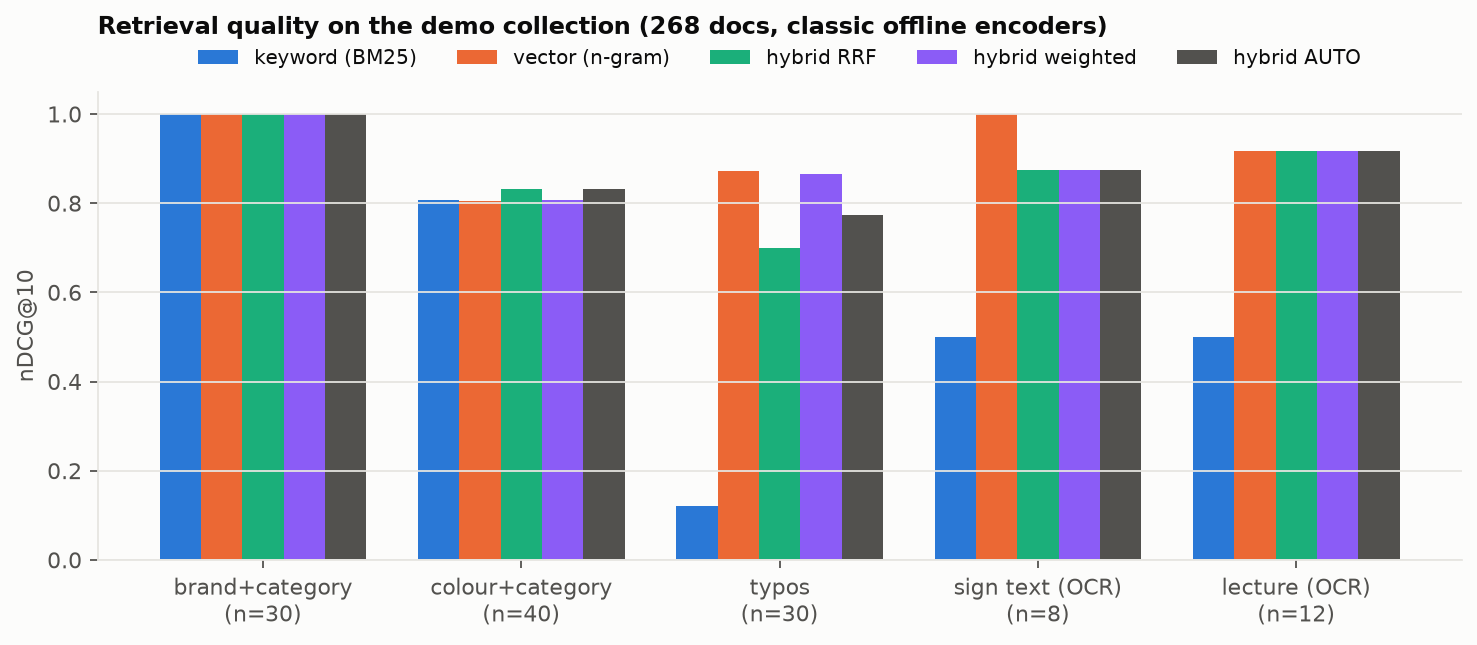
\includegraphics[width=\linewidth]{quality_demo.png}
\caption{nDCG@10 per query set and retrieval mode on the demo collection.}
\label{fig:quality}
\end{figure}

\begin{table}[H]
\centering\small
\begin{tabular}{llrrrrr}
\toprule
Query set & Mode & R@1 & R@10 & MRR@10 & nDCG@10 & p50 ms \\
\midrule
\multirow{5}{*}{\shortstack[l]{brand+category\\ \footnotesize $n=30$}} & Keyword (BM25) & 1.000 & 1.000 & 1.000 & \textbf{1.000} & 1.45 \\
 & Vector & 1.000 & 1.000 & 1.000 & \textbf{1.000} & 0.66 \\
 & Hybrid RRF & 1.000 & 1.000 & 1.000 & \textbf{1.000} & 2.09 \\
 & Hybrid weighted & 1.000 & 1.000 & 1.000 & \textbf{1.000} & 3.01 \\
 & Hybrid AUTO & 1.000 & 1.000 & 1.000 & \textbf{1.000} & 1.99 \\
\midrule
\multirow{5}{*}{\shortstack[l]{colour+category\\ \footnotesize $n=40$}} & Keyword (BM25) & 1.000 & 1.000 & 1.000 & 0.806 & 1.07 \\
 & Vector & 1.000 & 1.000 & 1.000 & 0.806 & 0.53 \\
 & Hybrid RRF & 1.000 & 1.000 & 1.000 & 0.831 & 1.51 \\
 & Hybrid weighted & 1.000 & 1.000 & 1.000 & 0.807 & 2.66 \\
 & Hybrid AUTO & 1.000 & 1.000 & 1.000 & \textbf{0.831} & 1.30 \\
\midrule
\multirow{5}{*}{\shortstack[l]{typos\\ \footnotesize $n=30$}} & Keyword (BM25) & 0.100 & 0.400 & 0.162 & 0.121 & 0.50 \\
 & Vector & 0.833 & 1.000 & 0.886 & \textbf{0.872} & 0.67 \\
 & Hybrid RRF & 0.800 & 1.000 & 0.859 & 0.700 & 1.12 \\
 & Hybrid weighted & 0.833 & 1.000 & 0.891 & 0.866 & 1.79 \\
 & Hybrid AUTO & 0.800 & 1.000 & 0.868 & 0.773 & 1.67 \\
\midrule
\multirow{5}{*}{\shortstack[l]{sign text (OCR)\\ \footnotesize $n=8$}} & Keyword (BM25) & 0.500 & 0.500 & 0.500 & 0.500 & 0.49 \\
 & Vector & 1.000 & 1.000 & 1.000 & \textbf{1.000} & 0.89 \\
 & Hybrid RRF & 0.875 & 0.875 & 0.875 & 0.875 & 1.02 \\
 & Hybrid weighted & 0.875 & 0.875 & 0.875 & 0.875 & 2.02 \\
 & Hybrid AUTO & 0.875 & 0.875 & 0.875 & 0.875 & 1.28 \\
\midrule
\multirow{5}{*}{\shortstack[l]{lecture (OCR)\\ \footnotesize $n=12$}} & Keyword (BM25) & 0.500 & 0.500 & 0.500 & 0.500 & 0.28 \\
 & Vector & 0.917 & 0.917 & 0.917 & \textbf{0.917} & 0.37 \\
 & Hybrid RRF & 0.917 & 0.917 & 0.917 & \textbf{0.917} & 0.87 \\
 & Hybrid weighted & 0.917 & 0.917 & 0.917 & \textbf{0.917} & 1.84 \\
 & Hybrid AUTO & 0.917 & 0.917 & 0.917 & \textbf{0.917} & 1.00 \\
\bottomrule
\end{tabular}

\caption{Retrieval quality on the demo collection. Bold: best nDCG@10 in each query set. Recall@$k$
counts a query as answered if any relevant document is in the top $k$.}
\label{tab:quality}
\end{table}

\paragraph{Clean queries are easy for every mode.} Brand+category queries score nDCG@10 = 1.000 in every
mode. Colour+category queries always find a relevant item at rank 1 (R@1 = 1.000), but nDCG@10 tops
out at 0.83: the third of the products whose title omits the colour are unreachable from text,
whatever the fusion. Text-to-pixel matching needs a cross-modal encoder (the CLIP profile).

\paragraph{Typos break the keyword path.} Keyword search answers only 40\% of the typo queries within
the top 10 (nDCG@10 0.121), while character $n$-grams still overlap and the vector path reaches 0.872.
Hybrid RRF falls to 0.700. The untouched category word (\emph{``t-shirt''}) makes BM25 return
confident but wrong-brand results, and rank-based fusion gives them the same weight as the correct
vector ranking. For \emph{``ace t-shirt''}, 4 of the 7 relevant items reach the top 10 with vectors
alone, but only 1 after RRF. Weighted fusion with max-normalisation (0.866) is far more robust,
because a low-scoring BM25 list contributes little.

\paragraph{OCR noise is the dominant real-world effect.} The OCR model reads \emph{NO PARKING} as the
single token \code{NOPARKING} and \emph{Node splits} as \code{Nodesplits}. The recognizer drops the
spaces between words, and enabling RapidOCR's space-character option does not change that. Keyword
search therefore answers only the sign texts whose words survived (\emph{exit}, \emph{stop},
\emph{one way}, \emph{sale}): nDCG@10 0.500 for signs and 0.500 for lecture slides. Worse, the query
word \emph{``no''} matches the product model numbers \code{NO-1144}, so BM25 ranks Nova products first
for \emph{``no parking''}. The $n$-gram vectors are indifferent to the missing spaces and answer every
sign query (1.000) and 11 of 12 lecture queries (0.917). The one miss, \emph{``cost models''}, fails
in every mode, because ``models'' also matches every product's ``Model'' code. Hybrid fusion recovers
most of the vector path's quality (0.875 and 0.917) without being told which path to trust.

\begin{table}[H]
\centering\small
\begin{tabular}{lrr}
\toprule
Top-10 neighbour shares the query's\ldots & Precision@10 & Chance \\
\midrule
Same colour & 0.718 & 0.125 \\
Same category & 0.865 & 0.200 \\
\bottomrule
\end{tabular}

\caption{Query-by-example on the colour-layout image vectors, \code{SIMILAR(image\_vec, DOC(id))}:
the fraction of the 10 nearest images (excluding the query) that share the query image's colour or
category, over 60 random product queries.}
\label{tab:qbe}
\end{table}

\paragraph{The image path works without any text.} Query-by-example on the colour-layout vectors
(\tab{tab:qbe}) returns neighbours of the same colour 72\% of the time (chance: 12.5\%) and the same
category 87\% of the time (chance: 20\%). The silhouette of a sneaker or a mug is captured by the
spatial colour layout, even though no text is involved.

\paragraph{Takeaway.} No single retrieval path wins everywhere. Lexical search is exact but brittle to
typos and OCR noise; the vector path is robust but can be confused by shared sub-strings. Fusion is the
safe default, and \emph{how} it fuses matters: on noisy keyword lists, score-aware weighted fusion
beats rank-only RRF.

% ---------------------------------------------------------------------
\subsection{Retrieval quality on public benchmarks}
\label{sec:public}

The engine includes loaders and an evaluation harness for
four public cross-modal benchmarks (\tab{tab:public}). For each benchmark, the harness ingests the
corpus with captions, OCR and transcripts on the keyword side and CLIP / CLAP on the vector side. It
then scores every caption query in the five modes of \sect{sec:quality} with Recall@\{1,5,10\}, MRR@10
and nDCG@10. The captions used as queries are never ingested, which avoids answer leakage.

\begin{table}[h]
\centering\small
\begin{tabularx}{\linewidth}{lllL}
\toprule
Benchmark & Modality & Test split & Notes \\
\midrule
Flickr30k~\cite{flickr} & image & 1{,}000 images $\times$ 5 captions & Karpathy split; the recommended headline benchmark \\
MS-COCO~\cite{coco} & image & 5{,}000 images $\times$ 5 captions & BLIP-base was fine-tuned on COCO captions, so keyword/hybrid scores are optimistic \\
MSR-VTT~\cite{msrvtt} & video & 1{,}000 videos (1k-A) & keyframes every 1\,s, multi-vector MaxSim \\
Clotho v2.1~\cite{clotho} & audio & 1{,}045 clips $\times$ 5 captions & Whisper + CLAP \\
\bottomrule
\end{tabularx}
\caption{Supported public benchmarks.}
\label{tab:public}
\end{table}

These runs need the neural model profile (PyTorch, OpenCLIP, BLIP, Whisper; several GB of weights)
and the datasets themselves, which require accepting their licences. Their results are not part of
this report: all numbers above come from data the project generates itself. The commands to
reproduce them are in Appendix~\ref{app:repro}.

% =====================================================================
\section{Discussion}
\label{sec:discussion}

\paragraph{The optimizer earns its keep.} No fixed access path is safe. The plan that is best without
a filter (HNSW) is $540\times$ worse at 0.1\% selectivity, and the plan that is best with a selective
filter (exact scan) loses at full selectivity. A cost model with measured unit costs and decent
selectivity estimates chose correctly at every point we tested. The estimates come first: the q-error
results show that the statistics behind the choice matter as much as the cost formulas.

\paragraph{Work vs.\ time.} WAND, NRA and HNSW do far less \emph{work} than their exhaustive
counterparts, but in an interpreted language they can still lose on \emph{time} to a vectorised scan.
The benchmarks therefore report work (postings scored, node expansions, sorted/random accesses)
alongside latency, so the algorithmic comparison stays meaningful and the constant factors stay visible.
In a compiled implementation, the crossovers in Figures~\ref{fig:optimizer} and~\ref{fig:filters}
would move toward the index-based plans.

\paragraph{Exactness of fusion is a real issue.} Fixed-depth fusion, the default in most hybrid search
systems, silently drops up to 31\% of the true top-50 when the lists disagree. TA gives exactness at a
cost close to fixed-depth merging.

\paragraph{Hybrid search helps when the paths disagree.} The quality study shows that the two
retrieval paths fail in different ways. The keyword index needs exact tokens. The $n$-gram vector
space tolerates typos and OCR noise but is blind to word boundaries and meaning. Fusion recovers most
of the better path's quality without knowing in advance which path that is.

% =====================================================================
\section{Limitations and future work}
\label{sec:limits}

\begin{itemize}
  \item \textbf{Speed.} The pure Python engine runs HNSW about 13$\times$ slower than FAISS per query.
        A C or Rust core for graph traversal, WAND and NRA is the obvious next step; the cost model
        would then simply re-calibrate.
  \item \textbf{Durability and concurrency.} The engine supports a single writer. The record store
        commits per insert, but index files are checkpointed by \code{save()} with no write-ahead log,
        and deletes are tombstones without compaction.
  \item \textbf{Filtered HNSW.} Under anti-correlated filters the index itself degrades; the optimizer
        avoids this by cost, but ACORN-style predicate-agnostic neighbour expansion~\cite{acorn} would
        fix the index.
  \item \textbf{Correlation-aware estimation.} Selectivities combine under independence; joint
        statistics or sampling would let the optimizer anticipate the correlation effect of
        \tab{tab:correlation}.
  \item \textbf{Evaluation.} Systems results use synthetic data, and real-data retrieval quality
        requires the neural profile and licensed datasets (\sect{sec:public}).
\end{itemize}

% =====================================================================
\section{Conclusion}

OmniSearch shows that hybrid multimodal search is best understood, and best engineered, as a database
system. It reduces every modality to text and vectors, gives each a proper index with statistics, and
puts a calibrated cost-based optimizer and exact top-$k$ fusion on top. The experiments confirm the
classic lessons in a new setting: access-path choice depends on selectivity and correlation, selectivity
estimates must be good for that choice to be right, and approximate aggregation can be replaced by
exact, instance-optimal algorithms at little cost.

% =====================================================================
\begin{thebibliography}{99}
\small
\bibitem{bm25} S.~Robertson and H.~Zaragoza. The probabilistic relevance framework: BM25 and beyond.
  \emph{Foundations and Trends in Information Retrieval}, 3(4), 2009.
\bibitem{wand} A.~Z.~Broder, D.~Carmel, M.~Herscovici, A.~Soffer and J.~Zien. Efficient query evaluation
  using a two-level retrieval process. In \emph{CIKM}, 2003.
\bibitem{hnsw} Y.~A.~Malkov and D.~A.~Yashunin. Efficient and robust approximate nearest neighbor search
  using hierarchical navigable small world graphs. \emph{IEEE TPAMI}, 42(4), 2018.
\bibitem{pq} H.~J\'egou, M.~Douze and C.~Schmid. Product quantization for nearest neighbor search.
  \emph{IEEE TPAMI}, 33(1), 2011.
\bibitem{fagin2001} R.~Fagin, A.~Lotem and M.~Naor. Optimal aggregation algorithms for middleware. In
  \emph{PODS}, 2001.
\bibitem{rrf} G.~V.~Cormack, C.~L.~A.~Clarke and S.~B\"uttcher. Reciprocal rank fusion outperforms
  Condorcet and individual rank learning methods. In \emph{SIGIR}, 2009.
\bibitem{milvus} J.~Wang et al. Milvus: A purpose-built vector data management system. In
  \emph{SIGMOD}, 2021.
\bibitem{adbv} C.~Wei et al. AnalyticDB-V: A hybrid analytical engine towards query fusion for
  structured and unstructured data. \emph{PVLDB}, 13(12), 2020.
\bibitem{acorn} L.~Patel, P.~Kraft, C.~Guestrin and M.~Zaharia. ACORN: Performant and
  predicate-agnostic search over vector embeddings and structured data. In \emph{SIGMOD}, 2024.
\bibitem{selinger} P.~G.~Selinger et al. Access path selection in a relational database management
  system. In \emph{SIGMOD}, 1979.
\bibitem{clip} A.~Radford et al. Learning transferable visual models from natural language
  supervision. In \emph{ICML}, 2021.
\bibitem{flickr} P.~Young, A.~Lai, M.~Hodosh and J.~Hockenmaier. From image descriptions to visual
  denotations. \emph{TACL}, 2, 2014.
\bibitem{coco} T.-Y.~Lin et al. Microsoft COCO: Common objects in context. In \emph{ECCV}, 2014.
\bibitem{msrvtt} J.~Xu, T.~Mei, T.~Yao and Y.~Rui. MSR-VTT: A large video description dataset for
  bridging video and language. In \emph{CVPR}, 2016.
\bibitem{clotho} K.~Drossos, S.~Lipping and T.~Virtanen. Clotho: An audio captioning dataset. In
  \emph{ICASSP}, 2020.
\end{thebibliography}

% =====================================================================
\appendix
\section{Reproducing the results}
\label{app:repro}

\noindent On Windows, use \code{mingw32-make} in place of \code{make}.
\begin{lstlisting}[language=bash]
make install                        # venv + dependencies
make test                           # 100 tests
make demo                           # 268-item demo collection (ffmpeg)
python -m benchmarks.run_all        # systems benchmarks (~20 min)
python -m benchmarks.demo_quality   # demo retrieval quality
python -m benchmarks.plots          # figures + results/SUMMARY.md
cd report && latexmk -pdf omnisearch_report.tex

# public benchmarks (neural models + datasets)
pip install -r requirements-models.txt
# place the Flickr30k images and Karpathy split under data/flickr30k
python -m benchmarks.retrieval_quality --dataset flickr30k --root data/flickr30k
\end{lstlisting}

\section{OmniQL quick reference}
\begin{center}\small
\begin{tabularx}{\linewidth}{>{\raggedright\arraybackslash}p{0.44\linewidth}L}
\toprule
Clause & Meaning \\
\midrule
\code{MATCH(field, 'text' [, weight=w])} & BM25 scoring clause on a text field \\
\code{SIMILAR(field, q [, weight, ef, nprobe])} & vector scoring; $q$ is \code{'text'}, \code{IMAGE()}, \code{AUDIO()}, \code{DOC()}, \code{VECTOR[...]} or a weighted sum \\
\code{CONTAINS(field, 'words')} & hard keyword filter (all terms present) \\
\code{=, !=, <, <=, >, >=, IN, BETWEEN, IS [NOT] NULL} & attribute filters combined with \code{AND} / \code{OR} / \code{NOT} under three-valued logic \\
\code{FUSE RRF(k) | WEIGHTED(norm) | AUTO} & fusion of the scoring clauses \\
\code{WITH (option=value, ...)} & optimizer overrides: \code{strategy} (exact, index, postfilter), \code{topk} (full, ta, nra, exhaustive), \code{keyword\_algo}, \code{filter\_access}, \code{ef}, \code{nprobe}, \code{depth} \\
\bottomrule
\end{tabularx}
\end{center}

\end{document}
